\clearpage
\section{曲线积分与曲面积分}
\setstretch{1.75}

\subsection{复习要点} \par

本章讲义的内容包括：
(1)~梳理不同类型积分之间的关联；
(2)~提示学习重点和易错点；
(3)~提示概念的物理意义，帮助理解和记忆（\textit{将用楷体字书写，不感兴趣可忽略}）.

为了方便串联，讲解顺序会与教材有所不同.

\subsubsection{第一型曲线积分、第一型曲面积分}\par

两种“第一型”积分都是标量积分，可分别视为\textbf{一元函数定积分}和\textbf{二重积分}的一种特殊应用.\par
先说\textbf{第一型曲线积分}，它的原理与一元函数定积分相同，只不过将积分区域从“直线”（区间）转到了“曲线”上.
则积分式中的$\d x$（即自变量的微小变化量）应改为$\d s$（即曲线弧长的微小变化量，称为\textbf{弧微分}或\textbf{弧长微元}）.
至于弧长微元应该如何表示，其实在计算平面曲线和空间曲线弧长的时候就学习过.

 \textit{物理意义：被积函数$f$代表曲线$L$的线密度，则积分值等于曲线的质量.}

(1)~设\textbf{积分曲线}$L$是平面曲线$y = y(x)~(a \le  x \le b)$，被积函数是$f(x,y)$，则第一型曲线积分的计算公式：
\begin{eq1}
\int_{L}f(x,y)~\d s = \int_{a}^{b} f(x,y(x))~ \sqrt{1 + [y'(x)]^2}~\d x
\end{eq1}

(2)~设\textbf{积分曲线}$L$是平面曲线，参数方程为$x=x(t)$，$y = y(t)$（$\alpha \le t \le  \beta$），被积函数是$f(x,y)$，则第一型曲线积分的计算公式：
\begin{eq1}
\int_{L}f(x,y)~\d s = \int_{\alpha}^{\beta} f(x(t),y(t)) ~\sqrt{[x'(t)]^2 + [y'(x)]^2}~\d t
\end{eq1}

(3)~设\textbf{积分曲线}$L$是空间曲线，参数方程为
$x = x(t)$，$y = y(t)$，$z =z(t)$（$\alpha \le t \le \beta$），被积函数是$f(x,y,z)$，则第一型曲线积分的计算公式：
\begin{eq1}
\int_{L} f(x,y,z) ~\d s =
\int_{\alpha}^{\beta} f(x(t),y(t),z(t)) ~\sqrt{[x'(t)]^2 + [y'(x)]^2 + [z'(t)]^2}~\d t \\[4.5mm]
\end{eq1}

\textbf{第一型曲面积分}的原理与\textbf{二重积分}相同，只不过将积分区域从“平面区域”转到了“曲面上的区域”.
则积分式中的$\d \sigma$应改为曲面的\textbf{面积微元}$\d S$.
面积微元的表示方法在上一章，计算空间曲面面积时提及.

\textit{物理意义：被积函数$f$代表曲面$S$的面密度，则积分值等于曲面的质量.}

(1)~设\textbf{积分曲面}$S$由方程$z = z(x,y)$，$(x,y) \in D$给出，被积函数是$f(x,y,z)$，则第一型曲面积分的计算公式：
\begin{eq1}
\iint_{S} f(x,y,z)~\d S =
\iint_{D} f(x,y,z(x))~\sqrt{1 + z_{x}^{2} + z_{y}^{2}}~\d x \d y
\end{eq1}

(2)~设\textbf{积分曲面}$S$由参数方程
$x =x(u,v)$，$y = y(u,v)$，$z = z(u,v)$，$(u,v) \in D$给出，
被积函数$f(x,y,z)$，则第一型曲面积分的计算公式：
\begin{eq1}
\iint_{S} f(x,y,z)~\d S =
\iint_{D} f(x(u,v),y(u,v),z(u,v))~\sqrt{EG - F^2} ~\d u \d v
\end{eq1}
其中，$E$、$F$和$G$的定义：
$$
\setstretch{1.25}
    \begin{cases}
        E = \bm{r}_u \cdot \bm{r}_u = x_u^2 + y_u^2 + z_u^2 \\
        F = \bm{r}_u \cdot \bm{r}_v = x_u x_v +y_u y_v + z_u z_v\\
        G = \bm{r}_v \cdot \bm{r}_v = x_v^2 + y_v^2 + z_v^2
    \end{cases} 
$$
\setstretch{1.75}


\subsubsection{第二型曲线积分}\par

“第二型”积分的研究对象不再是标量函数，而是向量函数，也就是要研究向量的某种“累积”性质.
不过，两种“第二型”积分区别较大，因此分成1.1.2和1.1.4两个小节来讲.
1.1.5小节作为补充内容，将讨论两种“第二型”积分如何在形式上统一.

\textbf{第二型曲线积分}的背景是变力做功问题. 
在学习时，不需要掌握严格定义（书上的定义看得我头晕）.
首先应掌握积分的“写法”.
设向量函数（也称\textbf{向量场}）$\bm{F}(x,y) = (P(x,y),~Q(x,y))$，
\textbf{积分路径}是\textbf{有向曲线}$L :\overset{\frown}{AB}$，
则$\bm{F}$沿$L$的第二型曲线积分可表示为：
\begin{eq1}
\int_{\overset{\frown}{AB}} P~\d x + Q ~\d y
~~~~\text{或}~~~
\int_{\overset{\frown}{AB}} \bm{F}(x,y) \cdot \d \bm{r}
\end{eq1}
其中$\d  \bm{r} = (\d x, \d y)$.
这个表示方法也可以扩展到三维（乃至$n$维），
只需将$\bm{F}$改为三维的向量函数$\bm{F}(x,y,z) = (P(x,y,z),~Q(x,y,z),~R(x,y,z))$即可，
此时$\d  \bm{r}$则是$(\d x, \d y, \d z)$.

\textit{设向量场$\bm{F} = (P,Q)$代表力，则力只与位移$\bm{r} = (x,y)$有关.
$L:\overset{\frown}{AB}$代表质点运动的轨迹.
则第二型曲线积分的值代表运动过程中力场对质点所做的功.
这个功可以理解为将力$\bm{F}$在每一段小位移$\d \bm{r}$上所做的“微功”$\d W$累积起来.
而“微功”则是$\bm{F}$与微小位移的点乘，即我们在积分式中所看到的$\bm{F}(x,y) \cdot \mathrm{d} \bm{r}$.
这个点乘的用向量坐标展开表示就成为了$P ~\d x + Q ~\d y$.
在$\mathbb{R}^3$中则是$P ~\mathrm{d} x + Q  ~\mathrm{d} y + R ~\mathrm{d} z$. } \vspace{1em}

第二型曲线积分有一条重要性质：若积分路径方向相反，则积分值的符号也相反，即：
\begin{eq1}
    \int_{\overset{\frown}{AB}} \bm{F}~\d \bm{r}
    =
    -\int_{\overset{\frown}{BA}} \bm{F}~\d \bm{r}
\end{eq1}

\textit{这反映了当位移量不变而位移方向相反时，做的功也会正负颠倒.}\par \vspace{1em}

关于第二型曲线积分的计算，事实上不需要记忆公式.
只需将曲线方程当做换元法的变量替换式，代入积分表达式中即可.
注意在代入$\d x$和$\d y$时，应遵循一节微分形式不变性的运算规则.
设曲线$L: \overset{\frown}{AB}$由参数方程$x = x(t)$，$y =y(t)$给出，参数$t$由$\alpha$变动到$\beta$，即$t=\alpha$对应起点$A$，$t = \beta$对应终点$B$.
则$\bm{F} = (P(x,y),Q(x,y))$沿$\overset{\frown}{AB}$的第二型曲线积分为：
\begin{eq1}
\int_{\overset{\frown}{AB}} P~\d x + Q ~\d y
&=
\int_{\alpha}^{\beta} P(x(t),y(t))~\d x(t) + 
Q(x(t),y(t))~\d y(t) \\
&= \int_{\alpha}^{\beta}
P(x(t),y(t))\cdot x'(t) + Q(x(t),y(t))\cdot y'(t) ~\d t
\end{eq1}

如果积分路径是空间曲线，计算方法类似，这里不再重复展示.
再次强调路径方向的问题：必须把代表起点的$\alpha$放在积分下限，代表终点的$\beta$放在积分上限，即便$\alpha > \beta$也是如此.

\subsubsection{格林公式、第二型曲线积分与路径无关的条件}

第二型曲线积分的积分路径$L$可以取成一条\textbf{简单闭曲线}，即积分路径起点与终点重合，构成一个“环”.
这样的积分称为\textbf{环路积分}.
从纯数学角度来讲，本节的内容主要关心一个平面区域内部的积分（二重积分）与其边界上的积分（环路积分）的关系.
\textit{从物理的角度来讲，我们的目光将不仅限于变力做功问题的计算，
而是要借助环路积分来研究向量场$\bm{F}$本身的性质——
例如，若$\bm{F}$代表重力场，一个质点沿环路运动一周回到原点的过程中，重力所做的总功是多少？}.

首先，我们对环路积分的方向表述做了规定.
很多时候，我们不会简单地只提“曲线$L$”，而是会强调它是某一区域$D$的边界.
在探讨“沿区域$D$的边界$L$的环路积分”时，我们以“正向”（记作$L^{+}$）和“负向”来区分两种不同的积分方向.
“正向”对外部边界而言是指逆时针方向，而对内部边界（即“洞”的边界）而言是指顺时针方向.
严格来说，对于一个有“洞”的区域$D$（即不是单连通区域），其边界$L$就不是“一个”环路，而是多个环路.
此时如果要直接计算$L$上的积分，需要分别按各自相应的方向对每个环路（包括外部边界和所有“洞”的边界）做积分，再相加.

之所以强调是对“区域$D$的边界”做积分，是因为要将区域内部和边界上的积分联系起来.
这就是\textbf{格林公式}的意义.
~\par \vspace{1em}
\textbf{定理（格林公式）}~~设函数$P(x,y)$，$Q(x,y)$在有界闭区域$D$上有连续的一阶偏导数，$D$的边界$L$是逐段光滑的，则有格林公式：
\begin{eq1}
\oint_{L^{+}} P~\d x + Q ~\d y = 
\iint_{D} \left( \frac{\partial Q}{\partial x} - \frac{\partial P}{\partial y} \right)~\d x \d y
\end{eq1} \par \vspace{1.2em}

“区域内有连续的一阶偏导数”这个条件十分重要.
在使用格林公式之前必须先验证这个条件，方可使用.
即便区域内仅有一个点不满足这个条件，也不能使用.
此事在教材8.3节的例3中亦有记载（考试很有可能考类似的题目）.\par \vspace{1em}

使用格林公式可以将环路积分转化为区域$D$内的二重积分，这对于考试时做计算题很有用.
但更重要的是，我们发现，如果区域$D$内向量函数（向量场）$\bm{F}$处处满足$\frac{\partial Q}{\partial x} = \frac{\partial P}{\partial y}$，则边界上环路积分的值的恒等于$0$.
\textit{在现实中，$\bm{F}$的具体例子可以是重力场$\bm{G}$和静电场$\bm{E}$——
物体在重力场$\bm{G}$中沿任何环路运动一周，重力所做的总功也都为$0$；
单位电荷在静电场$\bm{E}$中沿任何环路运动一周，电场力所做的总功都为$0$.
类似上面的场称为\textbf{保守场}，对应的力称为\textbf{保守力}.
}\par \vspace{0.5em}

对于单连通区域$D$，若$P(x,y)$和$Q(x,y)$在$D$内一阶偏导连续，则$\frac{\partial Q}{\partial x} - \frac{\partial P}{\partial y} = 0$除了等价于“$D$内环路积分恒等于$0$”之外，还有两个重要的等价表述：

(1)~$D$内任何第二型曲线积分的值都与路径无关，只与起点与终点的位置有关.
\textit{即：保守力对物体做的功只与物体的始末位置有关.}

(2)~$P ~\d x + Q~ \d y$恰是某个函数$u(x,y)$的全微分，即有$\d u(x,y) = P ~\d x + Q ~\d y$.
这个二元函数$u$称为$P ~\d x + Q ~\d y$的\textbf{原函数}.
注意，此时$\bm{F} = (P,Q)$其实就是$u(x,y)$的梯度，所以满足上述条件的向量场$\bm{F}$也称为\textbf{梯度场}.
更进一步，还有一个非常类似于牛顿莱布尼茨公式的结论：
\begin{eq1}
    \int_{\overset{\frown}{AB}} P ~\d x + Q ~\d y  = \int_{A}^{B} ~\d u = u(B) - u(A)
\end{eq1}

\textit{上述结论说明，对于保守力一定可以定义相应的势和势能.
例如，当$\bm{F}$为重力场$\bm{G}$，则原函数$u(x,y)$就代表重力势能.
物体运动时，重力所做的功等于物体始末位置的重力势能之差.
重力可以理解为重力势能的梯度.
}

\subsubsection{第二型曲面积分}\par

\textbf{第二型曲面积分}也是要对向量场做积分.
但是区别在于，第二型曲线积分是“沿着”曲线的方向做积分，
而第二型曲面积分是“垂直于”曲面的方向做积分.
因此在物理意义上就有很大的不同.
\textit{第二型曲面积分计算的是“流量”或“通量”这样的物理量.
书中举的例子是水流量. 
也可以通过电通量和磁通量来理解.}

我们的第一步是定义曲面的方向.
首先需注意，不是所有的曲面都是\textbf{双侧曲面}，例如\textbf{莫比乌斯带}就只有一个面.
不过现在我们不考虑这种离谱的曲面.
对于一个正常的双侧曲面，
我们可以给它“装备”一个法向量场$\bm{n}$，用以给曲面指定方向.
当法向量$\bm{n}$的$z$分量为正数，我们称选定了曲面的\textbf{上侧}；
当法向量$\bm{n}$的$z$分量为负数，我们称选定了曲面的\textbf{下侧}.
对于封闭曲面，我们也可以按直观简单地取“外侧”（记为$S^{+}$）和“内侧”作为两种不同的定向.
不过在计算时，我们归根结底还是要回到上侧与下侧的区别.
例如，若指定单位球面的方向是向外侧，对于上半球面而言这是指上侧，而对于下半球面这是指下侧.

第二型曲面积分的“写法”既反映“通量”的物理意义，又直接告诉了我们计算方法.
对于一个指定了方向的双侧曲面$S$，设曲面上每个点$(x,y,z)$上对应方向的单位法向量为$\bm{n}(x,y,z)$（注意一定是“单位”法向量）.
$\bm{F}(x,y,z) = (P(x,y,z),~Q(x,y,z),~R(x,y,z))$是曲面$S$上的向量函数（向量场）.
则$\bm{F} = (P,Q,R)$在$S$上的第二型曲面积分表示为：
\begin{eq1}
    \iint_{S} \bm{F}(x,y,z) \cdot \bm{n}(x,y,z)~\d S
    ~~~~\text{或}~~~
    \iint_{S} \bm{F}(x,y,z) \cdot \d \bm{S} 
\end{eq1}

此外，平时更多遇见的是用坐标形式来书写：
\begin{eq1}
    \iint_{S} P~\d y \d z + Q ~\d z \d x + R ~\d x \d y
\end{eq1}

三种写法相比，可见$\d ~ \bm{S} = \bm{n}(x,y,z)~\d S = (\d y \d z, \d z \d x , \d x \d y)$.
若遇到$S$为封闭曲面，应在积分号上加一个“圈”，写成$\oiint$.


\textit{设向量场$\bm{F}$代表磁感应强度$\bm{B}$，则第二型曲面积分的值就代表磁通量$\Phi$.
直观上就是磁感线通过曲面$S$的一种“流量”.}\par \vspace{1em}

和第二型曲线积分类似的，第二型曲面积分也有一条重要性质：若曲面的定向相反，则积分值的符号也相反.
即：
\begin{eq1}
    \iint_{S^{+}} \bm{F}\cdot \bm{n}~\d S
    =
    - \iint_{S^{-}} \bm{F} \cdot \bm{n}~\d S
\end{eq1} \par \vspace{1em}

关于第二型曲面积分的计算，其实基本原理在表达式里已经体现了.
积分式中的$\d S$其实就是之前提到的\textbf{面积微元}，所以我们完全可以将被积的向量函数$\bm{F}$与曲面的单位法向量$\bm{n}$做点乘，再对曲面$S$做第一型曲面积分即可.
不过我们的教材有点看不起这种方法.
对于曲面$S$由方程$z = f(x,y),(x,y)\in D$给出的情况，只需稍加推导就可以得出更简单的算法.
这是因为曲面的（并非单位）法向量可以简单地表示为向上：$(-f_x , -f_y, 1)$或向下：$(f_x , f_y , -1)$.
要将其转化为单位法向量$\bm{n}$，应当除以其模长$\sqrt{1 + f_x^{2} + f_{y}^{2}}$.
但是我们又有面积微元$\d S = \sqrt{1 + f_x^{2} + f_{y}^{2}} ~ \d \sigma$，一乘一除可以相互抵消.
于是得到了第二型曲面积分直接转为二重积分的简便算法：
\begin{eq1}
    \iint_{S} \bm{F}(x,y,z) \cdot \bm{n}(x,y,z)~\d S 
    &= \iint_{S} \bm{F}(x,y,z) \cdot \pm (-f_x , -f_y, 1)~\d \sigma \\
    &= \pm \iint_{D} P \cdot (-f_x) + Q \cdot (-f_y) + R ~\d \sigma
\end{eq1}

\clearpage

注意第二行的积分的区域$D$是指$(x,y)$所属的平面区域.
积分号前的“$\pm$”需要按照曲面$S$的定向来取：若向上则取正号，若向下则取负号.\par \vspace{1em}

如果曲面形状特殊，或者被积向量函数$\bm{F}$形式特殊，
可能也需要利用换元法.
设曲面$S$由如下的参数方程给出：$x = x(u,v)$，$y = y(u,v)$，$z = z(u,v)$，$(u,v) \in D$.
则曲面$S$的法向量可以表示为两个切向量的叉乘，即$\bm{r}_u \times \bm{r}_v = (x_u , y_u, z_u) \times (x_v , y_v , z_v)$.
之后的推导和之前类似.
$\bm{r}_u \times \bm{r}_v$的模长为$\sqrt{EG-F^2}$，
而参数方程下的面积微元表示为$\d S = \sqrt{EG - F^2}~\d \sigma$.
二者代入积分表达式中一乘一除两相抵消，因此有参数方程下第二型曲面积分直接转为二重积分的简便算法：
\begin{eq1}
    \iint_{S} \bm{F}(x,y,z) \cdot \bm{n}(x,y,z)~\d S 
    &= \pm \iint_{D} \bm{F} \cdot (\bm{r}_u \times \bm{r}_v) ~\d \sigma \\
    &= \pm \iint_{D} 
    \begin{vmatrix}
        P & Q & R  \\[-4pt]
        x_u & y_u & z_u \\[-4pt]
        x_v & y_v & z_v \\
    \end{vmatrix}
    ~\d \sigma
\end{eq1}

这里积分号前的“$\pm$”也需要按照曲面$S$的定向来取：若$\bm{r}_u \times \bm{r}_v$的方向与曲面的定向一致，则取正号，否则取负号.

（注：教材上给出的法向量$(A,B,C)$的计算公式是将所有分量直接展开了，看起来比较繁琐.
如果熟悉向量叉乘和三阶行列式计算的话，按$\bm{r}_u \times \bm{r}_v$来记忆应该会更轻松.）



\subsubsection{*“通量型”第二型曲线积分与格林公式}\par

（注：本小节将改写第二型曲线积分与格林公式的形式，以展现曲线积分和曲面积分的深层联系.
这个知识点不太可能直接考，但是中间的推导是教材上出现的内容.
可以按照自身需求选择是否跳过这一部分.）

之前我们看到，第一型的曲线积分和第一型曲面积分形式类似，
都是由“直”到“曲”的推广，\textit{而且都蕴含着“对密度求积分即得质量”的物理意义.}
但是第二型曲线积分和第二型曲面积分却很不同. 
前者是“沿着”曲线的方向，后者是“垂直于”曲面的方向.
\textit{前者是求“功”或“势能”，后者是求“通量”或“流量”.}
那么能否将二者统一一下呢？
例如，定义一种“垂直于”曲线方向的曲线积分，\textit{即用曲线积分计算平面上通过曲线的“流量”或“通量”}；
或者，定义一种“沿着”曲面方向的曲面积分？

后一种想法不太可行.
因为对于曲面上一点，切平面上的任何一个向量都可以是“方向向量”，因此“沿着曲面方向”的意义是不明确的.
而前一种想法不仅可行，而且具有普遍意义，可以按照着这个思路扩展至$n$维的第二型“超曲面”积分.
不过在这里我们暂且不把目光放那么远，还是来看看如何写“垂直于”曲线方向的第二型曲线积分.\par \vspace{1em}


运用与第二型曲面积分相同的思想，对于平面曲线$L$，可以通过$L$的单位法向量$\bm{n}$来指定曲线的定向为“上侧”或者“下侧”，
特别地，当$L$为封闭曲线，可以指定其方向为“外侧”（记为$L^{+}$）或“内侧”.
再设$L$上有平面向量函数$\bm{F}(x,y) = (P(x,y),Q(x,y))$.
则可以定义“通量型”第二型曲线积分为：
\begin{eq1}
    \int_{L} \bm{F}(x,y) \cdot \bm{n}(x,y) ~\d s
    ~~~~\text{或}~~~
    \int_{L} \bm{F}(x,y) \cdot \d \bm{s}
\end{eq1}
其中$\d \bm{s} = \bm{n}(x,y) \cdot \d s$.
可见这样定义的曲线积分形式与第二型曲面积分就一致了，\textit{而且也有“$F$穿过$L$的通量”的物理意义.}
同样地，当$L$为封闭曲线，应在积分号上加一个“圈”，写成$\oint$，表示环路积分.

在本篇讲义的后文中，将用“通量型”第二型曲线积分代指上述定义的积分，而之前所学的第二型曲线积分称为“做功型”.
注意，如果不加说明的话，“第二型曲线积分”一般都指后者.
考试会考的也是后者.\par \vspace{1em}

接下来我们导出“通量型”第二型曲线积分下的格林公式.
参照教材8.3节的例6.
设区域$D$的边界为闭曲线$L$，$L$指向外侧的单位法向量为$\bm{n}$.
定义在$D$及其边界上的向量函数$\bm{F} = (P(x,y),Q(x,y))$，
其中$P(x,y)$和$Q(x,y)$在$D$及其边界上有连续一阶偏导数.

现在要将$\bm{F}$沿$L^{+}$的“通量型”和“做功型”第二型曲线积分建立联系.
按照计算第二型曲面积分的思路，需要先表示出$\bm{n}$.
设沿$L^{+}$的切向量的方向余弦为$\cos \alpha$和$\cos \beta$，将单位方向向量顺时针旋转$90°$，就得到了单位外法向量$\bm{n} = (\cos \beta , -\cos \alpha)$.
于是：
\begin{eq1}
    \oint_{L^{+}} \bm{F} \cdot \bm{n} ~\d s
    &= \oint_{L^{+}} P \cos \beta - Q \cos \alpha ~\d s \\
    &= \oint_{L^{+}} P ~\d y - Q ~\d x
\end{eq1}

第二个等号成立是因为$\cos \alpha \cdot \d s = \d x$，$\cos \beta \cdot \d s = \d y$.
将$\d x$和$\d y$视为直角边，$\d s$视为斜边即可.

现在，第二个等号右侧的积分是“做功型”的第二型曲线积分了.
可以对其应用格林公式，得：
\begin{eq1}
    \oint_{L^{+}} \bm{F} \cdot \bm{n} ~\d s
    = \iint_{D} \left( \frac{\partial P}{\partial x} + \frac{\partial Q}{\partial y} \right) ~\d \sigma
\end{eq1}

这个公式也可以看作“通量型”的格林公式.
有了这个公式，我们立刻把它拿来跟接下来所学的\textbf{高斯公式}做比较.

\subsubsection{高斯公式}

\textbf{定理（高斯公式）}~~\textit{设空间区域$\Omega$的边界是分片光滑的封闭曲面$S$，
函数$P(x,y,z)$，$Q(x,y,z)$，$R(x,y,z)$在$\Omega \cup S$上有一阶连续偏导数，
则有高斯公式：}
\begin{eq1}
    \oiint_{S^{+}} \bm{F} \cdot \bm{n}~ \d S 
    =
    \oiint_{S^{+}} P~\d y \d z + Q ~\d z \d x + R ~\d x \d y 
    = \iiint_{\Omega} \left( \frac{\partial P}{\partial x} + \frac{\partial Q}{\partial y} + \frac{\partial R}{\partial z} \right) ~\d V
\end{eq1} \par \vspace{1.2em}

可以发现高斯公式与上面的“通量型”格林公式形式上十分相似.
也可以说后者就是二维空间中的高斯公式.
那么是否有一维的高斯公式呢？
不妨尝试一下.
设$\bm{F}$是$\mathbb{R}$上的函数$F(x)$，区间$I = [a,b]$.
所谓区间的“边界”，其实就是$a$和$b$这两个区间端点而已.
因此公式左侧不再有积分，而只是$F(a)$和$F(b)$这两个函数值.
但要注意区间的“边界”可以是需要定向的.
所谓“外法向”对左侧端点$a$而言是向左，即$-1$；而对右侧端点$b$而言是向右，即$1$.
因此公式左侧应写为$F(b) - F(a)$.
公式右侧，根据规律，被积函数应该是$\frac{\partial P}{\partial x}$，实际上也就是$F'(x)$.

到这里我们发现，“一维的高斯公式”就是微积分基本定理：
\begin{eq1}
    F(b) - F(a) = \int_{a}^{b} F'(x) ~\d x
\end{eq1} \par \vspace{1.2em}

以上说明了“通量型”格林公式与微积分基本定理都可以视为与高斯公式有相同的意义.
为了让三个公式的形式更统一（\textit{也让物理意义更加明确}），
引入nabla算子$\nabla$.
以$\mathbb{R}^3$中的情形为例（$\mathbb{R}^2$中的情形可视为在$z = 0$的子空间下讨论，$\mathbb{R}$中的情形可视为在$z = 0$，$y = 0$的子空间下讨论），nabla算子表示为
$\nabla = (\frac{\partial}{\partial x}, ~\frac{\partial}{\partial y}, ~\frac{\partial}{\partial z})$，
则高斯公式右侧的被积函数可以写成$\nabla \cdot \bm{F}$，即$\nabla$以向量点乘的形式作用于向量函数$\bm{F}$.
我们把$\nabla \cdot \bm{F}$称为\textbf{散度}，也记作div$ \bm{F}$.
高斯公式等三条公式的意义可以用文字简单地表述为：向量场$\bm{F}$通过区域边界的通量等于区域内部散度的积分.

\textit{散度可以看成区域内每一点附近极小体积内的流量或通量. 
如果将向量场比作水流（即每点处的$\bm{F}$视为该点水流的速度向量），则散度大于$0$表示该点附近水的流出多于流入，如同一个泉眼. 
因此这样的点形象地称为“源”.
而散度小于$0$的点相反，水的流入多于流出，如同一个地漏.
这样的点就称为“漏”.
通过整个区域边界的净流量，仅取决于区域内的“源”和“漏”有多少、有多大.
这是物质守恒定律的一种表达方式.
在电磁学中，静电场的“源”和“漏”即是正电荷和负电荷之所在，而磁场是无源无漏的.
这样就已经表达出麦克斯韦方程组的一部分含义了.
}

\subsubsection{斯托克斯公式}

\textbf{定理（斯托克斯公式）}~~\textit{设$S$为分片光滑的双侧曲面，其边界$L$是分段光滑的闭曲线.
假定在$S$上取定一侧的单位法向量为$\bm{n}$，再规定$L$的定向，使得$L$的定向与$\bm{n}$的指向构成右手系.
记$S^{+}$和$L^{+}$分别为给定上述定向后的$S$及$L$.
若$\bm{F}(x,y,z) = (P(x,y,z),Q(x,y,z),R(x,y,z))$在$R+L$上有一阶连续偏导数，则有斯托克斯公式：}
\begin{eq1}
    \oint_{L^{+}} P~\d x + Q~\d y + R ~\d z
    &= \iint_{S^{+}} 
    \begin{vmatrix}
        \d y \d z & \d z \d x & \d x \d y  \\
    \frac{\partial}{\partial x} & \frac{\partial}{\partial y} & \frac{\partial}{\partial z} \\
    P & Q & R    
    \end{vmatrix} \\
    &= \iint_{S^{+}} \left( \frac{\partial R}{\partial y} - \frac{\partial Q}{\partial z}\right) ~\d y \d z 
    + \left( \frac{\partial P}{\partial z} - \frac{\partial R}{\partial x}\right) ~\d z \d x
    + \left( \frac{\partial Q}{\partial x} - \frac{\partial P}{\partial y}\right) ~\d x \d y
\end{eq1} \vspace{1em}

将斯托克斯公式与格林公式放在一起比较：
\begin{eq1}
    \oint_{L^{+}} P~\d x + Q ~\d y = 
    \iint_{D} \left( \frac{\partial Q}{\partial x} - \frac{\partial P}{\partial y} \right)~\d x \d y
\end{eq1} \par 

二者形式也是非常相似的.
事实上，格林公式可以视作斯托克斯公式限制在$z = 0$子空间上的特殊情况（$R = 0$，$\d z = 0$）.
公式左侧都为第二型曲线积分，称为向量场$\bm{F}$沿$L$的\textbf{环量}.
而公式右侧，由上文引入的nabla算子，被积函数可以写成：
\begin{eq1}
    \begin{vmatrix}
        \bm{i} & \bm{j} & \bm{k}  \\
    \frac{\partial}{\partial x} & \frac{\partial}{\partial y} & \frac{\partial}{\partial z} \\
    P & Q & R    
    \end{vmatrix}
    = \left( \frac{\partial}{\partial x} , ~\frac{\partial}{\partial y} , ~\frac{\partial}{\partial z} \right)
    \times (P,Q,R)
    = \nabla \times \bm{F}
\end{eq1}
即$\nabla$与向量场$\bm{F}$以向量叉乘的形式相作用.
我们把$\nabla \times \bm{F}$称为\textbf{旋度}，也记作rot$\bm{F}$.
注意旋度是一个向量场而非标量场.
斯托克斯公式的意义可以用文字简单地表述为：
向量场$\bm{F}$在区域边界上的环量等于区域内部旋度的积分.

\textit{在计算右侧的第二型曲面积分时，被积分的rot$\bm{F}$还需与单位法向量$\bm{n}$点乘，才能转化为第一型曲面积分.
rot$\bm{F} \cdot \bm{n}$称为沿$\bm{n}$的\textbf{方向旋量}.
这个方向旋量可以理解为区域内每一点“自转”的程度.
这里仍然将向量场比作水流. 
若它在区域边界的环量非零，表明这片区域类似于一个“漩涡”，
而旋量非零的点如同漩涡的中心，因此形象地称为向量场的“旋”.
在电磁学中，磁场虽然无源无漏，但是有“旋”，而且“旋”的位置恰是激发磁场的电流所穿过的位置.
}

\subsection{解题方法}

\subsubsection{常规计算题}

\begin{example}{1}
    {
        设$\varGamma $是球面$x^2 + y^2 + z^2 =1$与平面$x=y$的交线，求$\oint_{\varGamma} (x^2 + y^2) ~\d s$的值.
    }
\end{example}    \vspace{0.5em}

\begin{remark}
    此为空间第一型曲线积分，为了转化为一元函数定积分，需要先写出$\varGamma$的参数方程.
\end{remark}  \vspace{0.5em}

\begin{solution}
    $\varGamma$的参数方程为：
    \[
    \begin{cases}
        x = \frac{1}{\sqrt{2}} \cos t \\
        y = \frac{1}{\sqrt{2}} \cos t ~~~~~~ t \in [0, 2\pi]\\
        z = \sin t \\
    \end{cases}
    \]

    计算弧微元：
    \begin{eq1}
        \d s = \sqrt{[x'(t)]^2+[y'(t)]^2+[z'(t)]^2} ~\d t 
        = \sqrt{\left( - \frac{1}{\sqrt{2}} \sin t \right)^2 
        + \left( - \frac{1}{\sqrt{2}} \sin t \right)^2
        + \cos^2 t} ~\d t 
        = \d t
    \end{eq1}

    代入积分：
    \begin{eq1}
        \oint_{\varGamma} (x^2 + y^2) ~\d s
        &= \int_{0}^{2\pi} \cos^2 t ~\d t \\
        &= \frac{1}{2} \int_0^{2 \pi} (1 + \cos 2t) ~\d t \\
        &= \pi
    \end{eq1} \qed
\end{solution}



\begin{example}{2}
    {
        设 \(\varGamma\) 是空间圆周
$
\begin{cases} 
    \setstretch{1.25}
x^2 + y^2 + z^2 = a^2 \\[-6pt]
x + y + z = \frac{3}{2}a 
\end{cases}
$（$a > 0$），计算
$
I = \oint_{\varGamma} (2yz + 2zx + 2xy) \, \d s
$
    } 
\end{example}\vspace{0.5em}
\setstretch{1.75}

\begin{remark}
    这题的做法比较取巧.
    提示同学们代入曲线方程时，注意被积函数与曲线之间的联系.
\end{remark} \vspace{0.5em}

\begin{solution}
    利用恒等式 \((x + y + z)^2 = x^2 + y^2 + z^2 + 2xy + 2yz + 2zx\)，并代入已知条件 \(x + y + z = \frac{3a}{2}\) 和 \(x^2 + y^2 + z^2 = a^2\)，积分可改写为：
    \begin{eq1}
    I
    &= \oint_{\varGamma} \left[ (x + y + z)^2 - (x^2 + y^2 + z^2) \right] \d s \\
    &= \oint_{\varGamma} \left[ \left( \frac{3a}{2} \right)^2 - a^2 \right] \d s = \frac{5a^2}{4} \oint_{\Gamma} 1 \, \d s
    \end{eq1}

    其中，\(\oint_{\varGamma} 1 \, ds\) 表示曲线 \(\varGamma\) 的周长.
    $\varGamma$是球面与平面相交得到的圆周.
    球心 \((0,0,0)\) 到平面的距离为：
    \[
    d = \left| \frac{0 + 0 + 0 - \dfrac{3a}{2}}{\sqrt{1^2 + 1^2 + 1^2}} \right| = \frac{\sqrt{3}}{2} a
    \]
    
    则圆 \(\varGamma\) 的半径为：
    $
    r = \sqrt{a^2 - \left( \frac{\sqrt{3}a}{2} \right)^2} = \frac{a}{2}.
    $
    圆 \(\varGamma\) 的周长即为$2\pi r = \pi a$.

    最终积分的结果为：
    \[
    I = \frac{5}{4} a^2 \cdot \pi a = \frac{5}{4} \pi a^3
    \] \qed
\end{solution}


\begin{example}
    {3}{
        求圆柱面 \( x^2 + y^2 = ax \) 在球 \( x^2 + y^2 + z^2 = a^2 \) 内的部分的面积.
    }
\end{example} \vspace{0.5em}

\begin{remark}
    求曲面的面积一般会用第一型曲面积分.
    但是对于曲顶柱面而言，用第一型曲线积分就够了.
\end{remark} \vspace{0.5em}

\begin{solution}
    首先将曲线方程转换为柱坐标下的参数方程：
    \begin{eq1}
        \setstretch{1.5}
        \begin{cases}
        r = a \cos\theta \\[-4pt]
        z = a \sin \theta
        \end{cases}
    \end{eq1}
    \setstretch{1.75}

   柱面在$xOy$上的投影曲线$L:~r = a \cos\theta$，$z=0$（图1）的弧微元为：  
   \begin{eq1}
   \d s = \sqrt{\left( \frac{dr}{d\theta} \right)^2 + r^2} \, d\theta = \sqrt{a^2 \sin^2\theta + a^2 \cos^2\theta} \, d\theta = a \, d\theta.
   \end{eq1}

   由于球内部分关于$xOy$平面对称，曲面的面积元素$\d A$就是：
   \begin{eq1}
       \d A = 2 \cdot |z| \cdot \d s = 
       2a^2 \sin \theta \, d\theta
   \end{eq1}

   则曲面面积$S$可以表示为第一型曲线积分：
   \begin{eq1}
      S = \int_{L} \d A &= 2 \int_{-\pi / 2}^{\pi / 2} 2a^2 | \sin \theta | ~\d \theta \\
      &= 4 \int_{0}^{\pi / 2} a^2 \sin \theta ~\d \theta \\
      &= 4a^2
   \end{eq1} \qed
\end{solution}

\begin{figure}[H] 
    \centering
    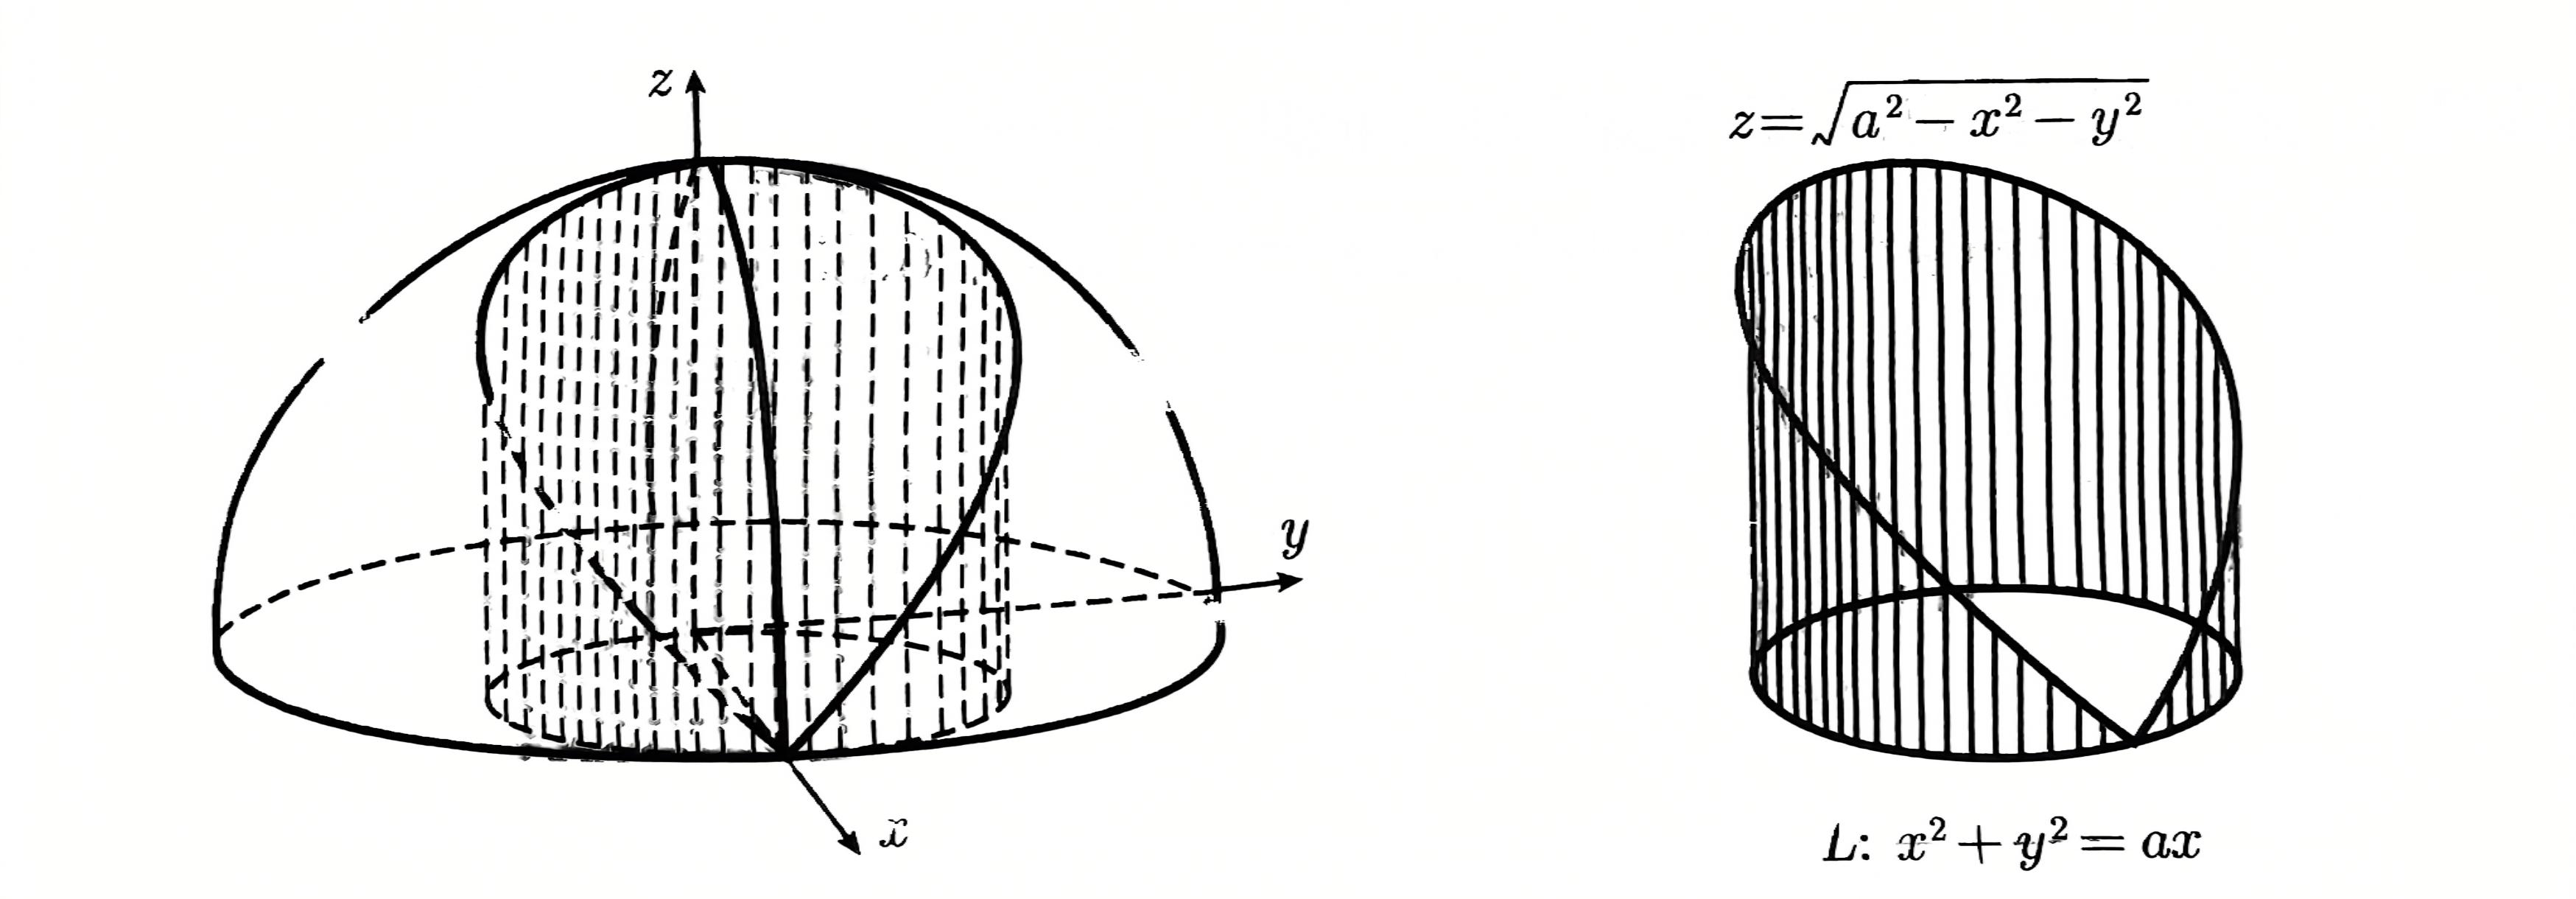
\includegraphics[width=1\textwidth]{fig8-1.jpg}
    \caption{例3曲面图} 
\end{figure}

\clearpage



\begin{example}
    {4(2021)}{
        计算曲面积分 
    $
    I = \iint_{\Sigma} \left( x^{2}y^{2} + y^{2}z^{2} + z^{2}x^{2} \right) \, \d S
    $.\vspace{0.5em}
    }
\end{example}
\begin{remark}
    这是一道平平无奇的第一型曲面积分.
    解答1和解答2分别展示曲面采用直角坐标方程和参数方程表示的做法，最终殊途同归.
\end{remark}  \vspace{0.5em}
\textbf{解答1（直角坐标系）}~~圆锥面方程为 \( z = \sqrt{x^{2} + y^{2}} \)，
投影区域 \( D \) 为 \( x^{2} + y^{2} \le 1 \).
为了计算面积微元$\d S$，先计算$z$的两个偏导数：
\begin{eq1}
    \frac{\partial z}{\partial x} = \frac{x}{\sqrt{x^{2} + y^{2}}} = \cos\theta, \quad \frac{\partial z}{\partial y} = \frac{y}{\sqrt{x^{2} + y^{2}}} = \sin\theta
\end{eq1}

则面积微元：
\begin{eq1}
    \d S = 
    \sqrt{1 + \left( \frac{\partial z}{\partial x} \right)^{2} + \left( \frac{\partial z}{\partial y} \right)^{2}} \, \d x \d y = \sqrt{2} \, \d x \d y
\end{eq1}

向$I$中代入曲面方程和面积微元，转化为$D:x^2 + y^2 \le 1$上的二重积分.
之后采用极坐标换元：
\begin{eq1}
    I &= \iint_{D} \left( x^2 y^2 + (x^2 + y^2)^2  \right) \cdot \sqrt{2}~ \d x \d y \\
    &= \sqrt{2} \iint_{D} \left( r^4 \cos^2 \theta \sin^2 \theta + r^4 \right)\cdot r~ \d r \d \theta \\
    &= \sqrt{2} \int_{0}^{2\pi} \d \theta \int_{0}^{1} r^{5}\left( 1 + \cos^{2}\theta\sin^{2}\theta \right) \, \d r \\
    &= \frac{\sqrt{2}}{6} \int_{0}^{2\pi} \left( 1 + \cos^2 \theta \sin^2 \theta \right) ~\d \theta \\
    &= \frac{\sqrt{2}}{6} \int_{0}^{2\pi} \left( 1 + \frac{1 - \cos 4\theta}{8}\right) ~\d \theta \\
    &= \frac{\sqrt{2}}{6} \int_{0}^{2\pi} \frac{9}{8} ~\d \theta \\
    &= \frac{\sqrt{2}}{6} \cdot \frac{9}{8} \cdot 2 \pi = \frac{3\sqrt{2} \pi }{8}
\end{eq1} \vspace{0.5em}

\textbf{解答2（参数方程）}~~将曲面$S$用参数方程表示：
$$
\setstretch{1.25}
    \begin{cases}
    x = r\cos\theta \\
    y = r\sin\theta \\
    z = r
    \end{cases} \quad (0 \le r \leq 1,\ 0 \leq \theta \leq 2\pi)
$$
\setstretch{1.75}

为了计算面积微元$\d S$，需先计算$E$，$F$和$G$：
$$
\setstretch{1.25}
    \begin{cases}
        E = x_r^2 + y_r^2 + z_r^2 = \cos^2 \theta + \sin^2 \theta + 1 = 2\\
        F = x_r x_\theta +y_r y_\theta + z_r z_\theta = -r \cos \theta \sin \theta + r \sin \theta \cos \theta =0 \\
        G = x_\theta^2 + y_\theta^2 + z_\theta^2 = r^2 \sin^2 \theta + r^2 \cos^2 \theta = r^2 
    \end{cases} 
$$
\setstretch{1.75}

则面积微元：
\begin{eq1}
    \d S = \sqrt{EG - F^2} ~\d r \d \theta = \sqrt{2} r ~\d r \d \theta
\end{eq1}

向$I$中代入曲面参数方程和面积微元，
转化为$D': 0 \le r \leq 1,\ 0 \leq \theta \leq 2\pi$
上的二重积分：
\begin{eq1}
    I = \iint_{D} \left( r^4 \cos^2 \theta \sin^2 \theta + r^4 \right)\cdot \sqrt{2} r~ \d r \d \theta = \frac{3\sqrt{2} \pi }{8}
\end{eq1} \qed \par
~\par

\begin{example}
    {5}{
        计算曲线积分$I = \oint_{L} y^2 ~\d x + z^2 ~\d y + x^2 ~\d z$.
        其中$L$是曲面$x^2 + y^2 = x$与与三维空间的单位球的交线在$z>0$的部分，
        方向是从$z$轴正向往负向看的逆时针方向.
    }
\end{example} \vspace{0.5em}

\begin{remark}
    此为第二型曲线积分，为了转化为一元函数定积分，需要先写出$L$的参数方程.
\end{remark} \vspace{0.5em}

\begin{solution}
    为了得到曲线$L$的参数方程，
    我们将单位球面和柱面$x^2 + y^2 = x$的方程都写成柱坐标的形式:
    \begin{eq1}
        \setstretch{1.25}
        \begin{cases}
            r^2 + z^2 =1 \\
            r = \cos \theta
        \end{cases}
    \end{eq1}

    \setstretch{1.75}

    由此我们可以通过$\theta$表示出$r=\cos \theta$和$z= \sin \theta$.
    如果我们想写出自变量$(x,y,z)$关于$\theta$的参数方程，
    还需要将$(x,y,z)$用柱坐标自变量$(r,\theta,z)$表示出来：
    \begin{eq1}
        \setstretch{1.25}
        \begin{cases}
            x = r\cos \theta = \cos^2 \theta \\
            y = r \sin \theta = \sin \theta \cos \theta \\
            z = |\sin \theta|
        \end{cases}
    \end{eq1}
    \setstretch{1.75}


为了计算曲线积分，我们需要对参数方程求导.
而考虑到 \(z\) 关于 \(\theta\) 的表达式带有绝对值，我们需要分 \(\theta\) 的符号计算导数：
\begin{eq1}
    \setstretch{1.25}
\begin{cases}
x'(\theta) = -\sin 2\theta \\
y'(\theta) = \cos 2\theta ~~~~~\theta \in \left[0, \frac{\pi}{2}\right]\\
z'(\theta) = \cos\theta
\end{cases}
~~~~~~
\begin{cases}
x'(\theta) = -\sin 2\theta \\
y'(\theta) = \cos 2\theta ~~~~~ \theta \in \left[-\frac{\pi}{2}, 0\right]\\
z'(\theta) = -\cos\theta
\end{cases}
\end{eq1}

代入公式计算第二型曲线积分：
\begin{align*}
    I &= \oint_L y^2 \d x + z^2 \d y + x^2 \d z \\
    &= \int_0^{\frac{\pi}{2}} \left( -\cos^2\theta \sin^2\theta \sin 2\theta + \sin^2\theta \cos 2\theta + \cos^5\theta \right) \d \theta \\
    &~~~~+ \int_{-\frac{\pi}{2}}^0 \left( -\cos^2\theta \sin^2\theta \sin 2\theta + \sin^2\theta \cos 2\theta - \cos^5\theta \right) \d \theta \\
    &= 2 \int_0^{\frac{\pi}{2}} \sin^2\theta \cos 2\theta d\theta \\
    &= 2 \int_0^{\frac{\pi}{2}} (\sin^2\theta - 2\sin^4\theta) d\theta = -\frac{\pi}{4} 
\end{align*}\qed 

\end{solution}
（摘抄xyt学长对此题的remark：
“特别指出，即便本题的曲线$L$关于$xOz$坐标平面对称，
这不意味着可以将积分分为$xOz$平面两侧的两段使用对称性计算积分，
因为第二型曲线积分累加的不是函数值而是向量函数和方向向量的内积，
内积的对称性是不直观的.
……
这一对称并不能保证第二型曲线积分所累积的内积$(y^2, z^2 ,x^2)\cdot (\d x,\d y,\d z)$是相反的，
因为关于$xOz$坐标平面对称的的两个点$A_1:(x_0,y_0,z_0)$和$A_2:(x_0, -y_0,z_0)$
的方向向量只有$x$分量$\d x$和$z$分量$\d z$是相反的，
方向向量的$y$分量$\d y$在对称点相同，
因此内积加和中项$y^2 \d x$和$x^2 \d z$
在$A_1$点和$A_2$点的值相反，
分量$z^2 \d y$
在$A_1$点和$A_2$点的值相同.
反映在定积分的计算中，
我们可以看到$x$和$z$分量的定积分是可以消去的，
$y$分量的则不行.”
）\par
~\par
\begin{example}
    {6}{
        求第二型曲面积分：
        $I = \iint_{S} (y-z)~\d y \d z + (z-x)~\d z \d x + (x-y) ~\d x \d y$.
        其中$S$是上半球面$x^2 + y^2 + z^2 = 2Rx ~(z \ge 0)$
        被柱面$x^2 + y^2 = 2rx$所截部分的上侧.
    }
\end{example} \vspace{0.5em}
\begin{remark}
    这道题展示第二型曲面积分化为第一型曲面积分的方法：既可以计算法向量直接转化，也可以用公式法.
    两种方法没有本质区别，一般推荐后一种.
\end{remark} \vspace{0.5em}

\begin{figure}[H] 
    \centering
    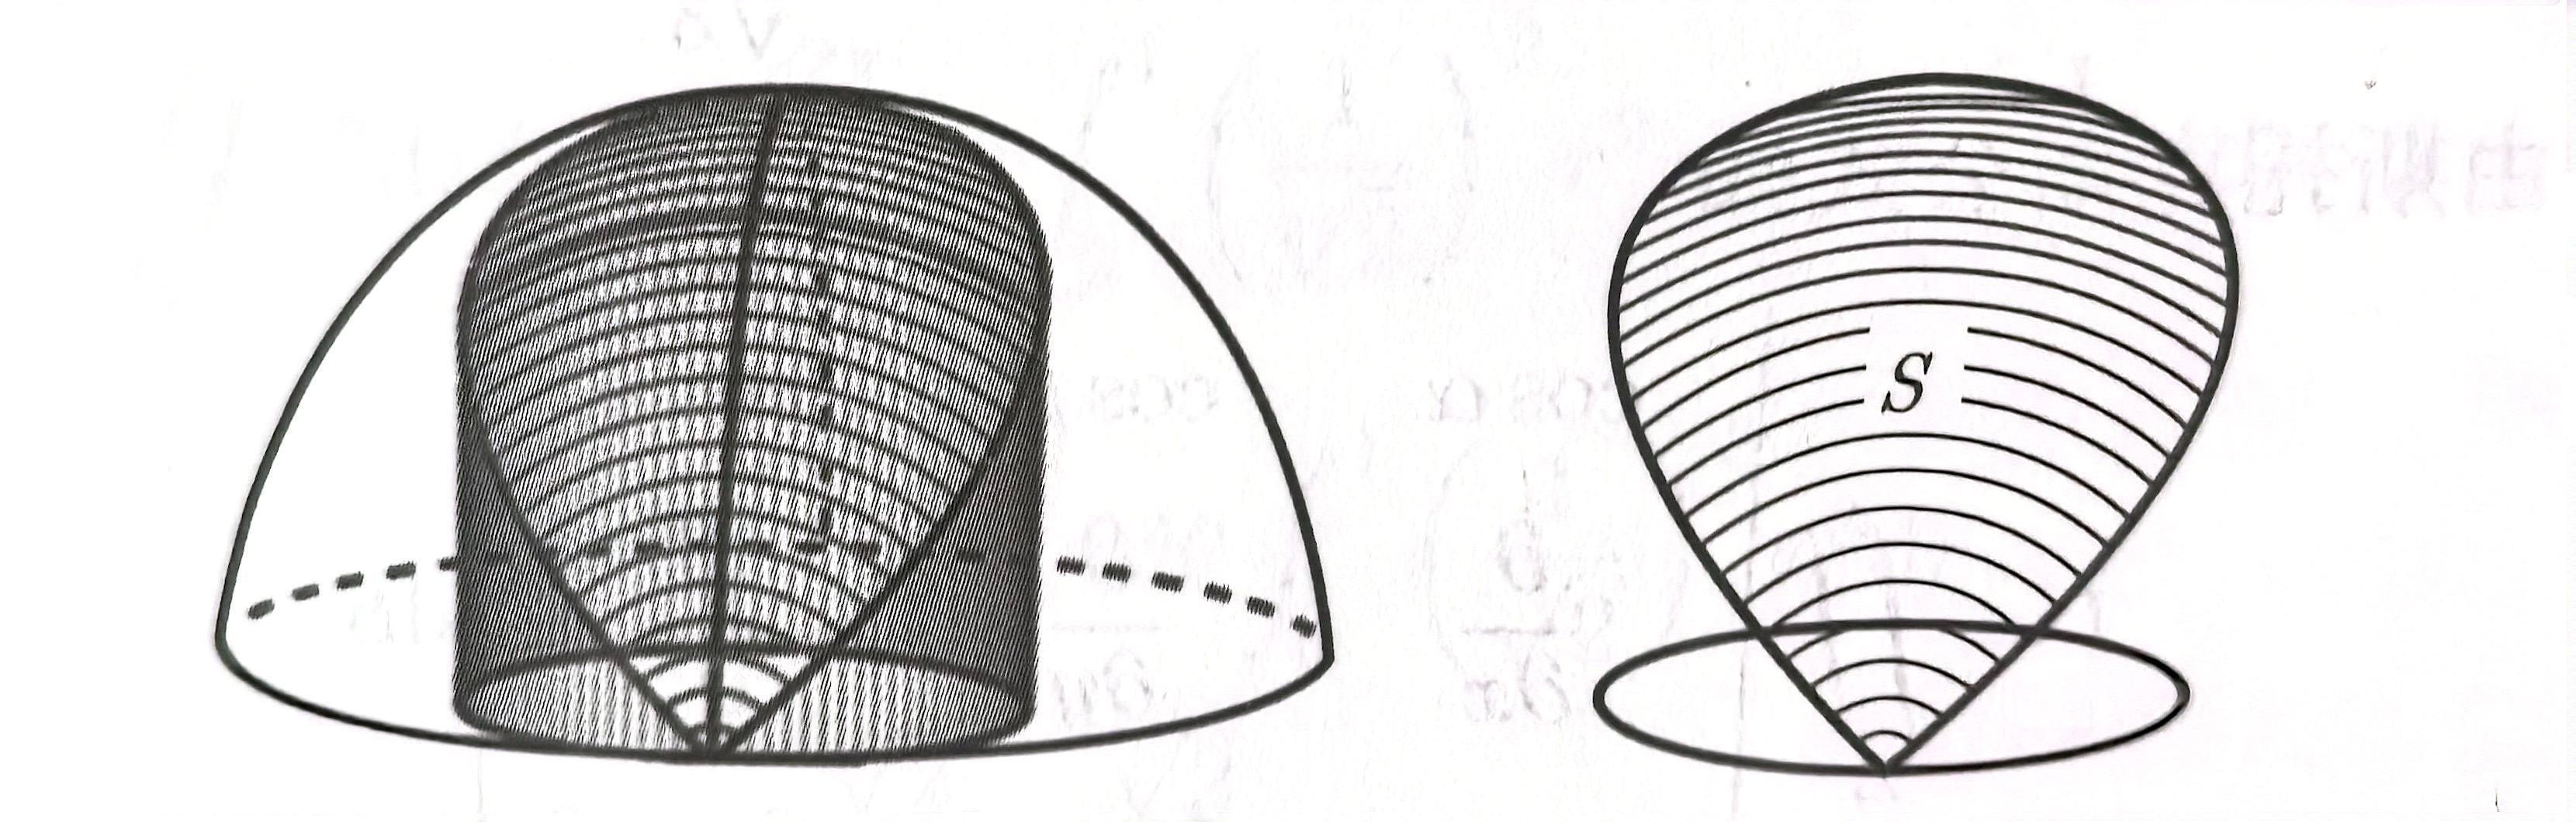
\includegraphics[width=0.8\textwidth]{fig8-2.jpg}
    \caption{例6曲面图} 
\end{figure}\par

\textbf{解答1（直接化为第一型曲面积分）}~~改写球面方程为：
\begin{eq1}
    (x-R)^2 + y^2 + z^2 = R^2
\end{eq1}

其外侧单位法向量$\bm{n} = (\frac{x-R}{R}, \frac{y}{R}, \frac{z}{R})$，将所求的第二型曲面积分转化为第一型曲面积分，即：

\begin{eq1}
    I = \iint_{S} \bm{F} \cdot \bm{n} ~\d S 
    &= \iint_{S} (y-z, z-x, x-y)\cdot (\frac{x-R}{R}, \frac{y}{R}, \frac{z}{R}) ~\d S \\
    &= \int_{S} (z-y) ~\d S  
\end{eq1}

因为$S$关于$xOz$平面对称，而函数$y$是关于$y$的奇函数，所以$\iint_{S} y ~\d S = 0$.
又$D_{xy}: x^2 + y^2 \le 2rx$的面积为$\pi r^2$.
于是有：
\begin{eq1}
    I = \int_{S} z ~\d S 
    &= \iint_{D_{xy}} \sqrt{2Rx - x^2 -y^2} \cdot \frac{R}{\sqrt{2Rx - x^2 -y^2}} ~\d x \d y \\
    &= R \int_{D_{xy}} ~\d x \d y = \pi r^2 R
\end{eq1}\qed

\textbf{解答2（公式法，直角坐标系）}~~改写球面方程为：
\begin{eq}
    z = f(x,y)= \sqrt{2Rx - x^2 - y^2}
\end{eq}

计算$z=f(x,y)$的偏导数：
\begin{eq1}
    f_x = \frac{R-x}{\sqrt{2Rx - x^2 - y^2}} = \frac{R-x}{z}
    ~,~
    f_y = \frac{-y}{\sqrt{2Rx - x^2 - y^2}} = \frac{-y}{z}
\end{eq1}

代入第二型曲线积分的公式（注意曲面定向是上侧）：
\begin{eq1}
    I &= \iint_{D_{xy}} (y-z, z-x, x-y) \cdot  (-f_x , -f_y, 1)~\d x \d y \\
    &= \iint_{D_{xy}} \frac{(x-R)(y-z)}{z} + \frac{y(z-x)}{z}+ \frac{z(x-y)}{z} ~\d x \d y \\
    &=\iint_{D_{xy}} \left(R - \frac{y}{z} \right) ~\d x \d y = \pi r^2 R  
\end{eq1} \qed 

~\par

\begin{example}
    {7}{
        求$\iint_{S} \frac{x~\d y \d z + z^2 ~\d x \d y}{x^2 + y^2 +z^2}$，
        其中$S$为柱面$x^2 + y^2 = R^2$及$z=-R$，$z=R$所围成的立体表面外侧.
    }
\end{example} \vspace{0.5em}

\begin{remark}
    $P = \frac{x}{x^2 + y^2 + z^2}$和$R = \frac{z^2}{x^2 + y^2 + z^2}$
    在$(0,0,0)$处不连续，不能用高斯公式.
    因此还得转化为二重积分计算.
    本题的曲面包括三部分：底面$S_1$，$S_2$和侧面$S_3$（图3），需要分别计算.
    注意可以利用曲面特殊的位置关系来简化积分.
    例如$S_1$和$S_2$是水平的平面，则其上的$P \d y \d z$恒为$0$，
    只需要计算$R ~\d x \d y$的积分即可.
    又如$S_3$是竖直的曲面，则其上的$R ~\d x \d y$恒为$0$，
    只需要计算$P ~\d y \d z$的积分即可.

    \begin{figure}[H] 
        \centering
        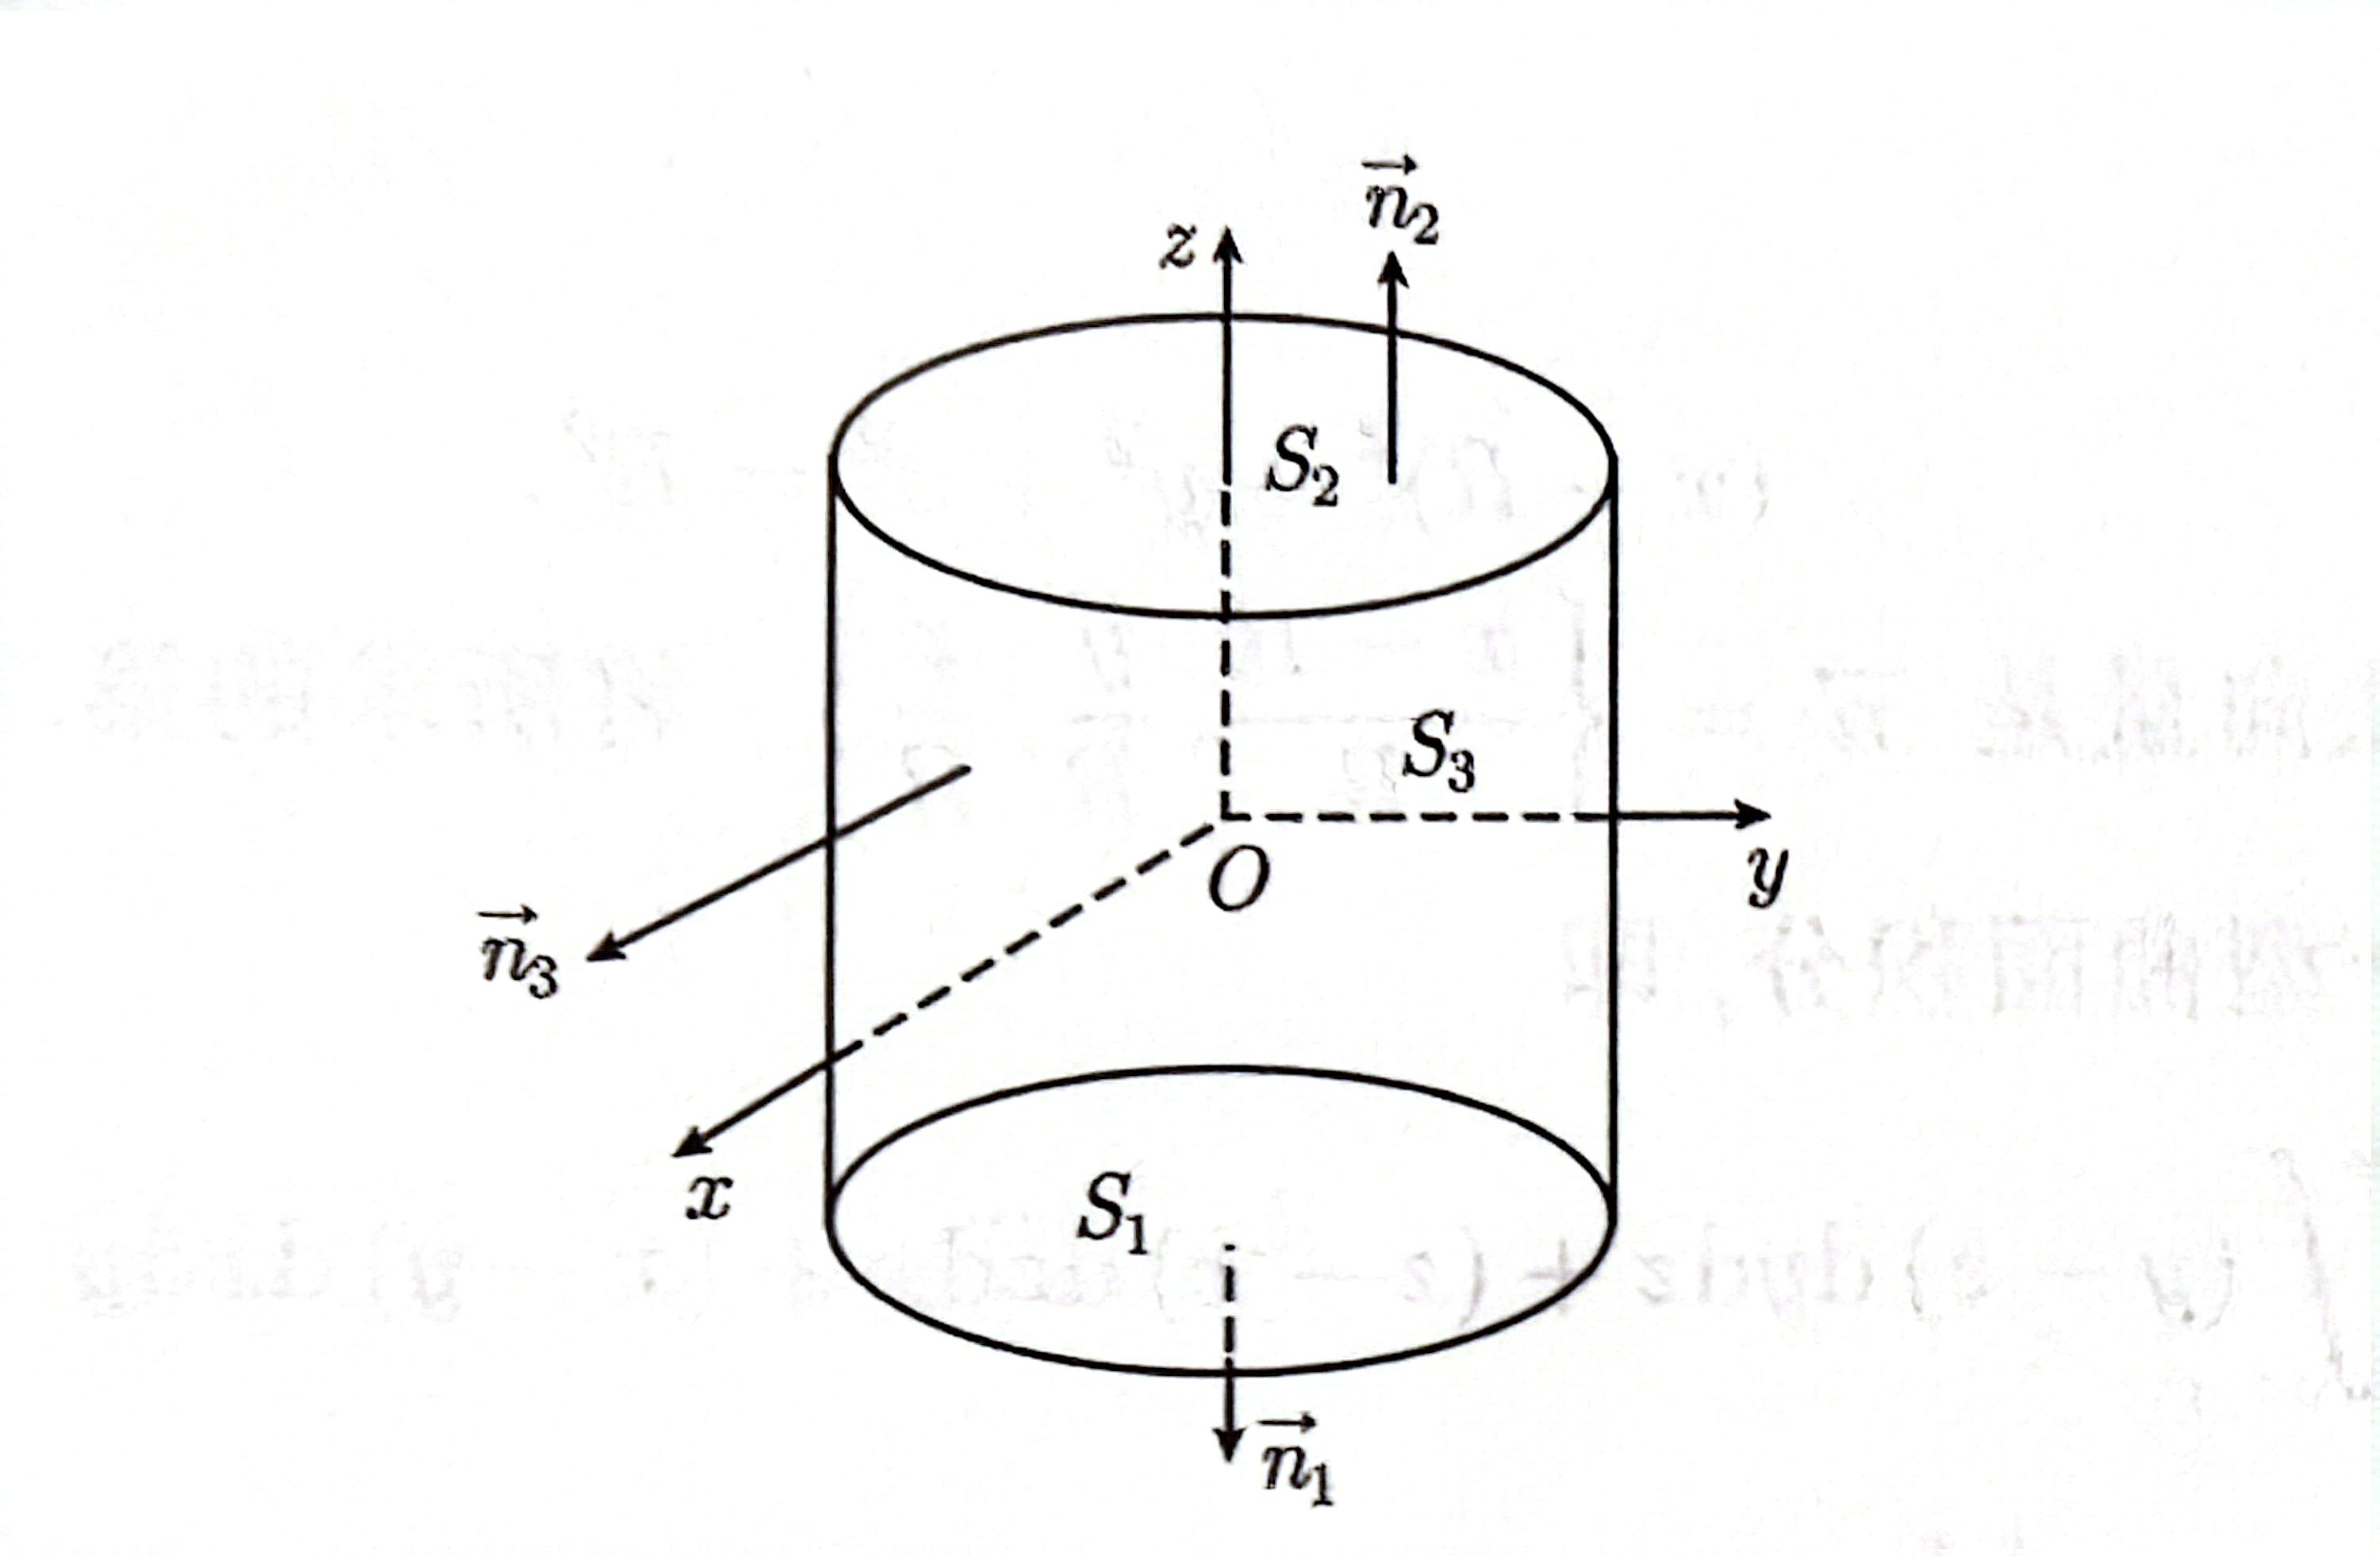
\includegraphics[width=0.5\textwidth]{fig8-3.jpg}
        \caption{例7曲面图} 
    \end{figure}\par

\end{remark}
\begin{solution}
    将所求积分拆项为：
    \begin{eq1}
        \iint_{S} \frac{x~\d y \d z + z^2 ~\d x \d y}{x^2 + y^2 +z^2}
        = \iint_{S} \frac{x~\d y \d z}{x^2 + y^2 +z^2}
        + \iint_{S} \frac{z^2 ~\d x \d y}{x^2 + y^2 + z^2}
    \end{eq1}

    先看第一项：
    \begin{eq1}
        \iint_{S_1} \frac{x ~\d y \d z}{x^2 + y^2 + z^2} = \iint_{S_2} \frac{x~ \d y \d z}{x^2 + y^2 + z^2} = 0 ~~\text{（注意  $\d y \d z = 0$）}
    \end{eq1}

    $S_3$为柱面$S_3 : x = \pm \sqrt{R^2 - y^2}$，
    它到$yOz$的投影面$D_{yx}$为：
    \begin{eq1}
        \setstretch{1.25}
            D_{yz} : 
\begin{cases}
-R \leq y \leq R \\
-R \leq z \leq R
\end{cases}
    \end{eq1}
    \setstretch{1.75}

    则第一项在$S_3$上的积分：
    \begin{eq1}
        \iint_{S_3} \frac{x ~\d y \d z}{x^2 + y^2 + z^2} 
        &= \iint_{S_3 \text{前}} \frac{\sqrt{R^2 - y^2} ~\d y \d z}{R^2 + z^2} + \iint_{S_3 \text{后}} \frac{ - \sqrt{R^2 - y^2} ~\d y \d z}{R^2 + z^2} \\
        &= \iint_{D_{yz}} \frac{\sqrt{R^2 - y^2} ~\d y \d z}{R^2 + z^2} - \iint_{D_{yz}} \frac{\sqrt{R^2 - y^2} ~\d y \d z}{R^2 + z^2} \\
        &= 2 \iint_{D_{yz}} \frac{\sqrt{R^2 - y^2}~\d y \d z}{R^2 + z^2} \\
        &= 2 \int_{-R}^{R} \frac{1}{R^2 + z^2} \d z \int_{-R}^{R} \sqrt{R^2 - y^2} \d y\\
        &= 8 \int_{0}^{R} \frac{1}{R^2 + z^2} \d z \int_{0}^{R} \sqrt{R^2 - y^2} \d y \\
        &= 8 \cdot \frac{1}{4} \pi R^2 \cdot \frac{\pi}{4R} = \frac{1}{2} \pi^2 R
    \end{eq1}

    再看第二项：
    \begin{eq1}
        S_1 : z = -R,~~D_{xy} : x^2 + y^2 \le R^2 \\
        S_2 : z = R, ~~D_{xy} : x^2 + y^2 \le R^2
    \end{eq1}

    \begin{eq}
        \iint_{S_1 + S_2} \frac{z^2 ~\d x \d y}{x^2 + y^2 + z^2} 
        = \iint_{D_{xy}} \frac{R^2}{x^2 + y^2 + R^2} ~\d x \d y 
        - \iint_{D_{xy}} \frac{R^2}{x^2 + y^2 + R^2} ~\d x \d y  = 0
    \end{eq}
    \begin{eq1}
        \iint_{S_3} \frac{z^2 ~\d x \d y}{x^2 + y^2 + z^2}  = 0 ~~\text{（注意  $\d x \d y = 0$）}
    \end{eq1}

    综上所述，原积分的值为$\frac{1}{2}\pi^2 R $. \qed
\end{solution}

~\par

\subsubsection{利用对称性简化计算}

第一型积分要化成一元函数定积分和重积分来计算，
因此对称性的利用和第三章、第七章所讲述过的类似.
这里通过几个例子再熟悉一下.\par
~\par

\begin{example}
    {8}{
        设$S$为空间中的单位球面$x^2 + y^2 + z^2 = 1$.
        计算曲面积分：$I = \iint_{S} (x+y+z)^2 ~\d S$.
    }
\end{example} \vspace{0.5em}
\begin{remark}
    曲面$S$具有完美的对称性.
    将被积函数展开：
    \begin{eq}
        (x+y+z)^2 = x^2 + y^2 + z^2 + 2xy + 2yz + 2zx
    \end{eq}
    
    可知后三项都是奇函数，在曲面$S$上的积分为$0$，故可以直接从积分中划去.
\end{remark} \vspace{0.5em}

\begin{solution}
    \begin{eq1}
        I &= \iint_{S} x^2 + y^2 + z^2 + 2xy + 2yz + 2zx ~\d S \\
        &=  \iint_{S} x^2 + y^2 + z^2 ~\d S \\
        &= \iint_{S} ~\d S = 4\pi
    \end{eq1} \qed
\end{solution} 

~\par

\begin{example}
    {9(2022)}{
        设 \( E \) 是椭圆 \(\{(x,y) \in \mathbb{R}^2 \mid x^2 + \frac{y^2}{4} = 1, -1 \leq x \leq 1, -2 \leq y \leq 2\}\).
        求第一型曲线积分 \(\int_E |xy| \, \d s\)
    }
\end{example} \vspace{0.5em}

\begin{remark}
    被积函数带绝对值，则是关于$x$和$y$的偶函数.
    而椭圆关于$x$轴和$y$轴对称.
    因此只需计算第一象限内的积分，再乘$4$即可.
    这样也自然地拆开了绝对值符号.
\end{remark} \vspace{0.5em}

\begin{solution}
    \( E \) 的参数方程为 \( x = \cos t \)，\( y = 2 \sin t \)，其中 \( 0 \leq t \leq 2\pi \).
    由对称性得：

\begin{eq1}
    \int_E |xy| \, \d s 
    &= 4 \int_0^{\frac{\pi}{2}} xy \, \sqrt{(\cos t)^2 + (2 \sin t)^2} \, \d t \\
&= 4 \int_0^{\frac{\pi}{2}} 2 \cos t \sin t \, \sqrt{\sin^2 t + 4 \cos^2 t} \, \d t \\
&= 4 \int_0^{\frac{\pi}{2}} \sin 2t \, \sqrt{1 + 3 \cos^2 t} \, \d t \\
&= 4 \int_0^{\frac{\pi}{2}} \sin 2t \, \sqrt{\frac{5}{2} + \frac{3}{2} \cos 2t} \, \d t 
\end{eq1}

令 \( u = \cos 2t \)，则 \( \d u = -2 \sin 2t \, \d t \)，
所以上述积分等于：\vspace{0.5em}
\begin{eq1}
    \int_E |xy| \, ds 
    &= -2 \int_1^{-1} \sqrt{\frac{5}{2} + \frac{3}{2}u} \, du = 2 \int_{-1}^1 \sqrt{\frac{5}{2} + \frac{3}{2}u} \, \d u \\
    &= 2 \left[ \frac{2}{3} \cdot \frac{2}{3} \left( \frac{5}{2} + \frac{3}{2}u \right)^{\frac{3}{2}} \right]_{-1}^1 \\
    &= \frac{8}{9} \left( 4^{\frac{3}{2}} - 1^{\frac{3}{2}} \right) = \frac{56}{9}
\end{eq1} \qed 
\end{solution}

~\par

\begin{example}
    {10}{
        设 \(\varGamma\) 为圆周
$
\begin{cases} 
    \setstretch{1.25}
    x^2 + y^2 + z^2 = a^2 \\[-6pt]
    x + y + z = a 
\end{cases}
$（$a > 0$），
计算空间第一型曲线积分：
$\oint_{\varGamma} x^2 ~\d s$. \vspace{0.5em}
    }
\end{example} \vspace{0.5em}

\begin{remark}
    本题的曲线$\varGamma$关于$(x,y,z)$有轮换对称性.
    借鉴第七章利用轮换对称性进行组合积分的思路.
\end{remark} \vspace{0.25em}


\begin{solution}
    由轮换对称性知：
    \begin{eq1}
        \oint_{\varGamma} x^2 ~\d s 
        = \oint_{\varGamma} y^2 ~\d s 
        = \oint_{\varGamma} z^2 ~\d s 
    \end{eq1}

    所以：
    \begin{eq1}
        \oint_{\varGamma} x^2 ~\d s 
        = \frac{1}{3} \oint_{\varGamma} (x^2 + y^2 + z^2)~\d s
        = \frac{a^2}{3} \oint_{\varGamma} ~\d s  
    \end{eq1}


其中$\oint_{\varGamma} ~\d s $即为$\varGamma$的全长.
$\varGamma$是平面$x+y+z=a$上的圆周，点$O(0,0,0)$到此平面的距离$d = \frac{a}{\sqrt{3}}$.
所以$\varGamma$的半径为：
\begin{eq1}
    R = \sqrt{a^2 - \left( \frac{a}{\sqrt{3}}\right)^2 } = \frac{\sqrt{6}}{3}a
\end{eq1}

所以：
\begin{eq1}
    \oint_{\varGamma} ~\d s = 2 \pi R = \frac{2\sqrt{6}}{9} \pi a^2  
\end{eq1} \qed

\end{solution} \vspace{0.5em}

第二型积分涉及向量值函数，在研究对称性时，需要综合考虑三点：

(1)被积函数的对称性；

(2)（曲线/曲面）的对称性；

(3)曲线单位方向向量/曲面单位法向量方向的对称性（对称点上是同向还是反向）.

不同分量的对称性质可能亦有不同，因此在使用时需要谨慎地检查.
最保险的方法是画出曲线/曲面的图来，在它的一组对称点上标出曲线/曲面的定向，
再标出被积函数的分量.
这样虽然麻烦，但是如果用对了，相比于不顾对称性死算一切题目还是有很大的时间优势.~\par
~\par

\begin{example}
    {11}{
        计算曲线积分$\oint_{L} \frac{\d x + \d y}{|x|+|y|}$.
        其中$L$其中$L$是由四个点
        $(2,0)$，$(-2,0)$，$(0,2)$和$(0,-2)$围成的正方形的边界的逆时针方向.
    }
\end{example} \vspace{0.5em}

\begin{solution}
    正方形边界$L$关于原点$O$中心对称.
    考虑$L$上任意关于$O$中心对称的两个点$A_1(x_0,y_0)$和$A_2(-x_0,-y_0)$.
    在这两点处沿$L$的单位方向向量$\bm{t}$平行反向，而
    被积函数$\bm{F} = (P(x,y),Q(x,y)) = \left(\frac{1}{|x|+|y|}, \frac{1}{|x|+|y|}\right)$
    在这两点的取值是相同的.
    故内积$\bm{F} \cdot \bm{t}$在对称点上互为相反数，相互抵消.
    可知：
    \begin{eq1}
        \oint_{L} \frac{\d x + \d y}{|x|+|y|}
        = \oint_{L} \bm{F} \cdot \bm{t} ~\d s = 0
    \end{eq1} \qed
\end{solution}

~\par

\textbf{例12(2023)}~~\textit{设曲面 \( S \) 是柱体  
    $\Omega = \{(x,y,z) \mid x^2 + y^2 \leq 1, \, 0 \leq z \leq 1\}$
    表面的外侧（同时包含上表面、下表面、侧面）.
    计算下列积分：}
    
    \textit{(a)} $I_1 = \iint_S (y - z) |x| \, \d y \, \d z + (z - x)|y| \, \d z \, \d x + (x - y)|z| \, \d x \, \d y$.\vspace{0.25em}
    
    \textit{(b)} $I_2 = \iint_S (y - z)x^2 \, \d y \, \d z + (z - x)y^2 \, \d z \, \d x + (x - y)z^2 \, \d x \, \d y$.\vspace{0.25em}
    
    \textit{(c)} $I_3 = \iint_S (y - z)x^3 \, \d y \, \d z + (z - x)y^3 \, \d z \, \d x + (x - y)z^3 \, \d x \, \d y$.\vspace{0.75em}

\begin{remark}
    这道题可以利用高斯公式简化计算.
    但在这里我们先展示不使用高斯公式的做法.
    关键是仔细分析图形和被积函数$\bm{F}$的对称性.
\end{remark} \vspace{0.5em}

\begin{solution}
    我们将$\Omega$的上表面，下表面和侧面分别记为$S_1$，$S_2$和$S_3$：
    \begin{eq1}
        S_1 &= \{ (x,y,z) \mid x^2 + y^2 \le 1, z=1 \} \\
        S_2 &= \{ (x,y,z) \mid x^2 + y^2 \le 1, z=0 \} \\
        S_3 =& \{ (x,y,z) \mid x^2 + y^2 = 1, 0 \le z \le 1 \}
    \end{eq1}
\end{solution}

故$S$上的第二型曲面积分$I$总是可以分解为：
\begin{eq1}
    I = \iint_{S_1+S_2} P~\d y \d z + Q~\d z \d x + R ~\d x \d y
    + \iint_{S_3} P~\d y \d z + Q~\d z \d x + R ~\d x \d y
\end{eq1}

由于$S_1$和$S_2$是垂直于$z$轴的平面，其上的$\d y \d z = \d z \d x =0$；
又因为$S_3$的法向量处处垂直于$z$轴，其上的$\d x \d y =0$.
故积分中可以先消去一些项：
\begin{eq1}
    I = \iint_{S_1+S_2} R~\d x \d y
    + \iint_{S_3} P~\d y \d z + Q ~\d z \d x 
\end{eq1}

接下来分析每个小问：\vspace{0.5em}

$\bm{(a)}$~~
\begin{eq1}
    I_1 = \iint_{S_1+S_2} (x-y)|z|~\d x \d y
    + \iint_{S_3} (y-z)|x|~\d y \d z + (z-x)|y| ~\d z \d x 
\end{eq1}

对于$S_1$和$S_2$上的积分，
只需分别代入$z=0$和$z=1$，
就转化成了单位圆$D_{xy}$上的二重积分.
而$x-y$是关于$x$和$y$的奇函数，因此：
\begin{eq1}
    \iint_{S_1} (x-y)|z|~\d x \d y
    = \iint_{S_2} (x-y)|z|~\d x \d y
    = 0
\end{eq1}

$S_3$上的积分涉及到两个分量.
以对$x$分量的积分为例，即计算：
\begin{eq1}
    \iint_{S_3} (y-z)|x|~\d y \d z
\end{eq1}

我们考虑$\bm{F}$以“前后”方向“穿入”或“穿出”的对称性.
即：考虑$S_3$上任意关于$yOz$平面对称的两个点$A_1(x_0,y_0,z_0)$和$A_2(-x_0,y_0,z_0)$.
在这两个点上，
曲面$S_3$上的单位法向量也是关于$yOz$对称的（与$x$轴的夹角余弦恰好相反）.
而$P = (y-z)|x|$是关于$x$的偶函数，在$A_1$点和$A_2$点的取值相同.
直观地说，如果向量场$\bm{F}$在$A_1$点“穿入”了$S_3$，
则它在与之对称的$A_2$点必然会以相同的$x$分量“穿出”，从而通量相互抵消.
这说明：
\begin{eq1}
    \iint_{S_3} (y-z)|x|~\d y \d z
    &= \iint_{S_{3\text{前}}} (y-z)|x|~\d y \d z + 
    \iint_{S_{3\text{后}}} (y-z)|x|~\d y \d z
    = 0 
\end{eq1}
同理可知：
\begin{eq1}
    \iint_{S_3} (z-x)|y| ~\d z \d x
    &= \iint_{S_{3\text{左}}} (z-x)|y| ~\d z \d x + 
    \iint_{S_{3\text{右}}}(z-x)|y| ~\d z \d x
    = 0 
\end{eq1}
故$S_3$上的积分为$0$.
综上所述，$I_1 =0$.\vspace{0.5em}

$\bm{(b)}$~~基于与$(a)$完全相同的理由，$I_2 = 0$.

$\bm{(c)}$~~基于与$(a)$完全相同的理由，我们依然能得到：
\begin{eq1}
    \iint_{S_1} (x-y)|z|~\d x \d y
    = \iint_{S_2} (x-y)|z|~\d x \d y
    = 0
\end{eq1}

不过在$S_3$上的情况似乎复杂了一些，
因为$P = (y-z)x^3$关于$x$是奇函数而不是偶函数了，
因此在关于$x$对称的方向上不能相互抵消.
对于$Q = (z-x)y^3$也是如此.
但是柱面关于$(x,y)$的对称性实在太好，
我们还可以找到其它的对称性来应对.

对于$x$分量上的积分，虽然$x$的对称性没有帮助了，但是还可以用$y$的对称性.
考虑$S_3$上关于平面$xOz$的一组对称点$B_1(x_0,y_0,z_0)$和$B_2(x_0,-y_0,z_0)$.
曲面$S_3$在这两点处的单位法向量与$x$轴的夹角余弦相同，而$P = (y-z)x^3$关于$y$是奇函数，
因此在这两点处取值恰好互为相反数，因而“穿入”和“穿出”相互抵消.
即：
\begin{eq1}
    \iint_{S_3} yx^3 ~\d y \d z =0
\end{eq1}

同理：
\begin{eq1}
    \iint_{S_3} (z-x)y^3 ~\d z \d x = 0
\end{eq1}

故$S_3$上的积分化简为：
\begin{eq1}
    \iint_{S_3} (y-z)x^3 ~\d y \d z + (z-x)y^3 ~\d z \d x =
    \iint_{S_3} -z x^3 ~\d y \d z + zy^3 ~\d z \d x 
\end{eq1}

观察剩余的这两部分积分：
\begin{eq1}
    \iint_{S_3} z x^3 ~\d y \d z~~,~~
    \iint_{S_3} zy^3 ~\d z \d x 
\end{eq1}

我们发现二者是完全相同的，只不过$x$和$y$交换了位置.
因此，这两个积分可以视为只有字母记号上的变化，
实际上还是同一个积分.
因此得到：
\begin{eq1}
    \iint_{S_3} -z x^3 ~\d y \d z + zy^3 ~\d z \d x =0
\end{eq1}

综上所述，$I_3 = 0$. \qed \par

\subsubsection{利用格林公式、高斯公式和斯托克斯公式转化}

我们学习的格林公式、高斯公式和斯托克斯公式，对于积分计算的帮助很大.
在考试中一般也会设置这样的题目类型：

(1)格林公式可以将第二型（封闭）曲线积分转化为二重积分；

(2)高斯公式可以将第二型（封闭）曲面积分转化为三重积分；

(3)斯托克斯公式可以将第一型（封闭）曲线积分转化为第二型曲面积分.

因此利用好这三个公式可以将难做的积分类型转化为好做的积分类型.
在应用这些公式时需要注意两点：

(1)注意这些公式本身也是定理，
因此在使用之前需要特别检查是否符合定理的前置条件.
这三个公式的共同点是要求被积函数\textbf{一阶连续可偏导}，也是最容易挖坑的点.
我们将在例题中着重反映这个问题.

(2)这些公式都是对封闭曲线/封闭曲面成立的.
但是并不意味着只有遇到封闭曲线/封闭曲面的积分时才会想到用这些公式.
对于不封闭的曲线/曲面，我们可以补加一段曲线/一片曲面，
使之变为封闭的，再代入公式.
最后减去我们所补加的部分即可.\par
~\par

\begin{example}
    {17}{
        求$I= \int_{L} (x+y)^3 ~\d x - (x-y)^3 ~\d y$，
        其中$L$为图$4$所示的两个上半圆周连成的曲线$AOB$.
    }
\end{example}

\begin{figure}[H] 
    \centering
    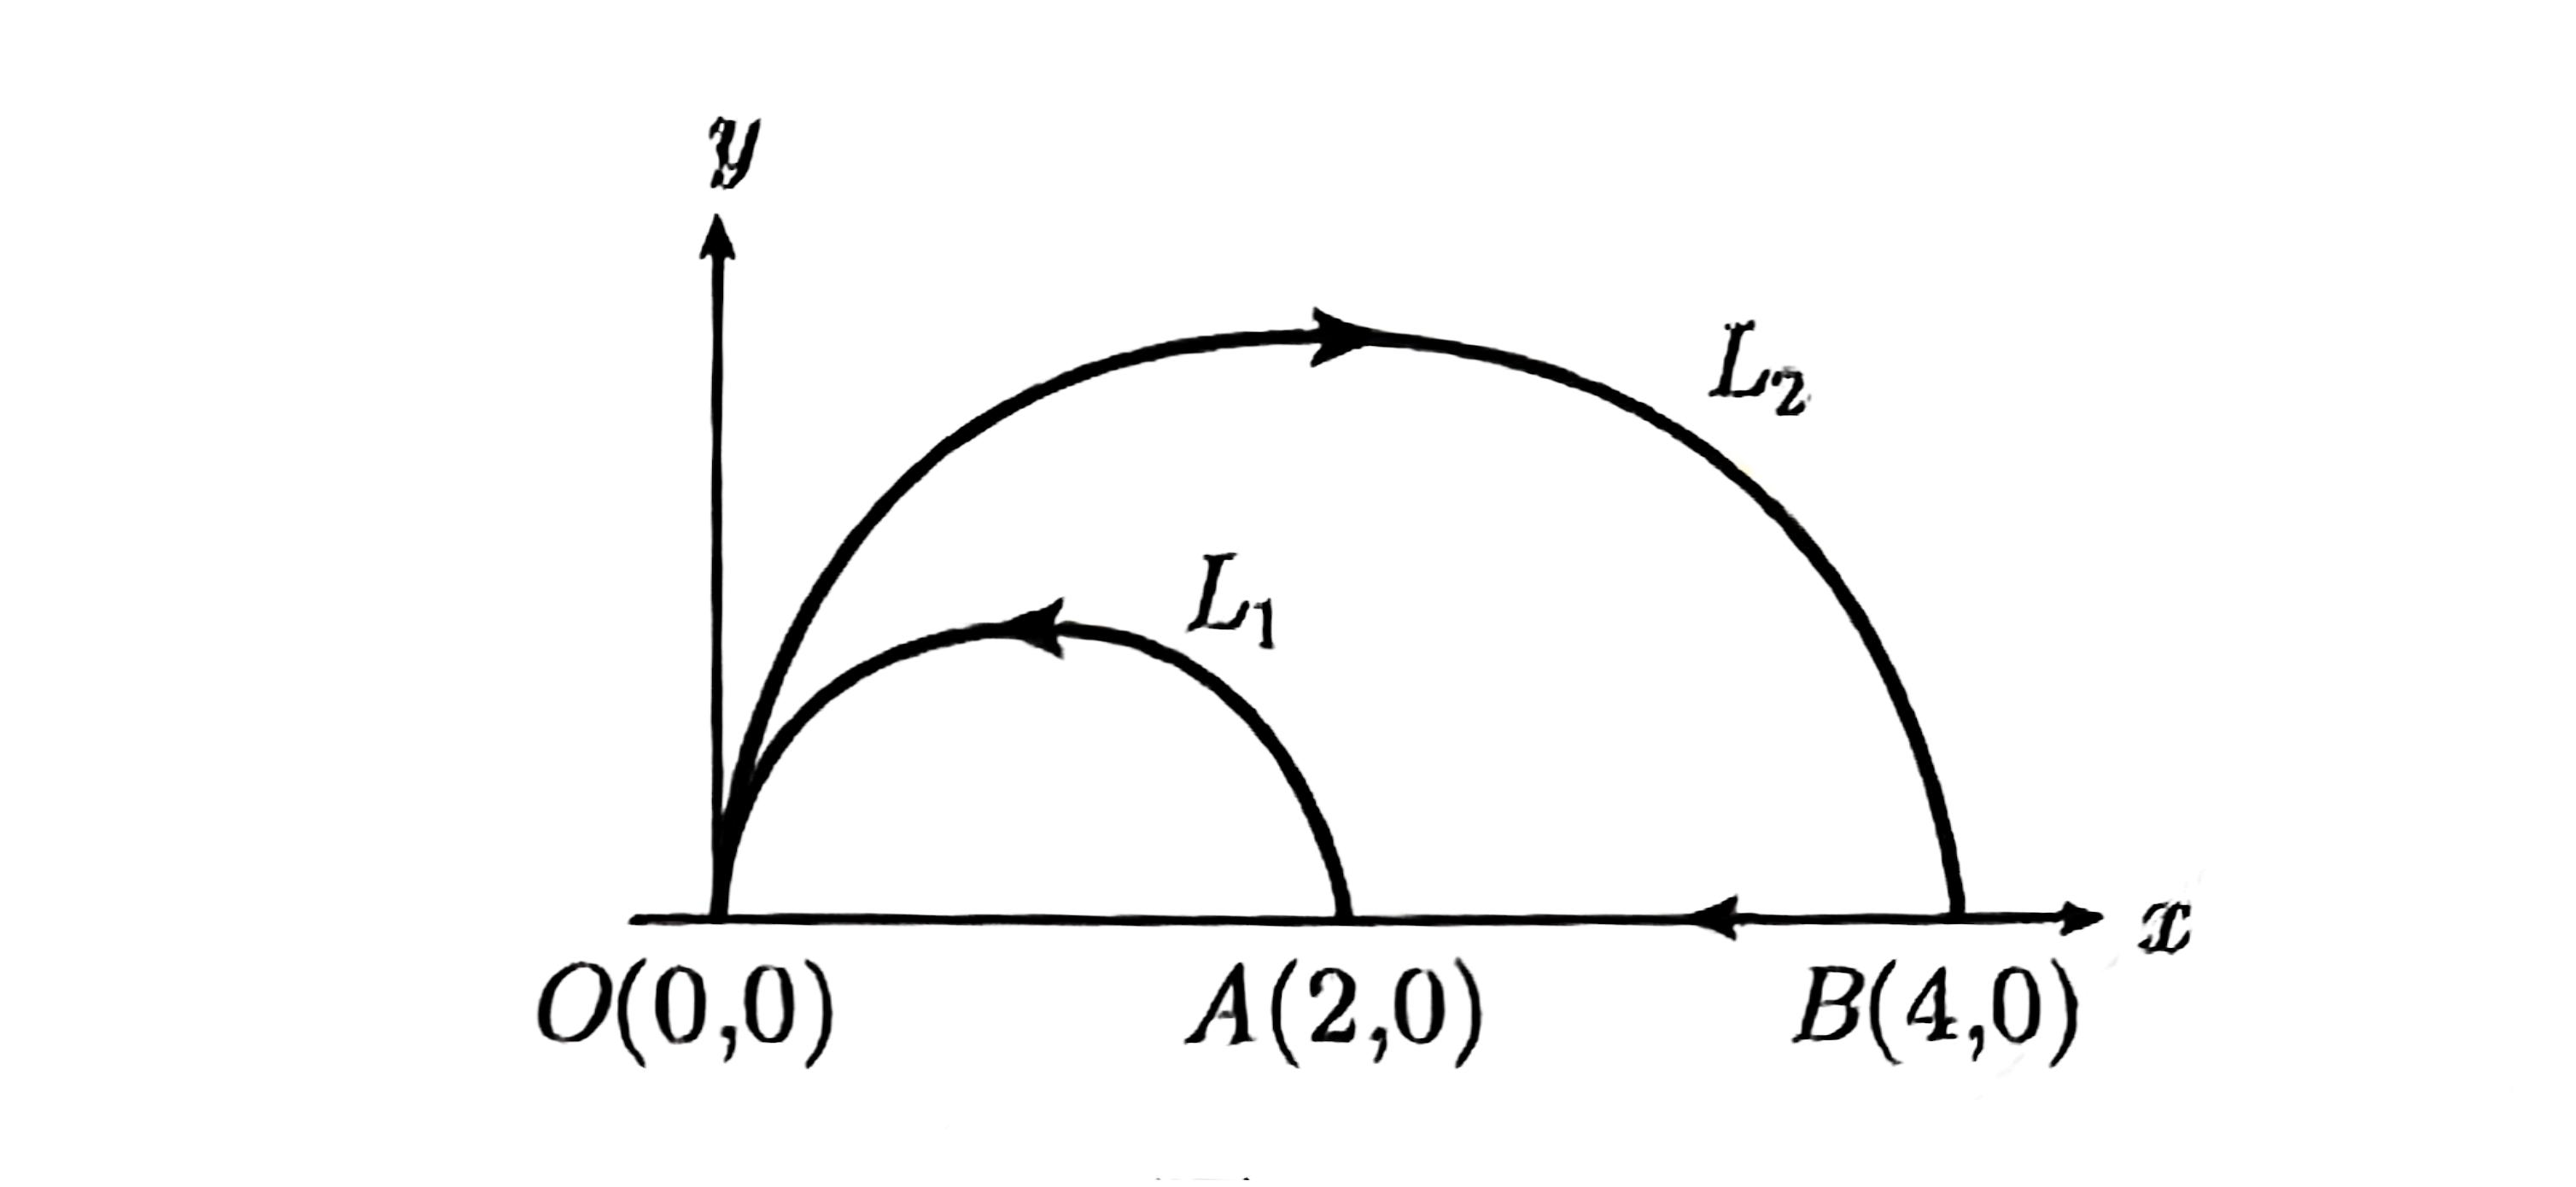
\includegraphics[width=0.5\textwidth]{fig8-4.jpg}
    \caption{例17题图} 
\end{figure}\par

\begin{remark}
    此题直接计算比较麻烦.
    而将其连成闭合回路只需连接$AB$.
    因此利用格林公式转化成二重积分可能是一个更好的选择.
\end{remark} \vspace{0.5em}

\begin{solution}
    记$P(x,y) = (x+y)^3$，$Q(x,y) = -(x - y)^3$.
    则有：
    \begin{eq1}
        \frac{\partial}{\partial x}Q(x,y) - \frac{\partial}{\partial y} P(x,y) 
        &= -3(x-y)^2 - 3(x+y)^2 \\
        &= -6x^2 - 6y^2 
    \end{eq1}

    添加有向线段$\overrightarrow{BA}$，
    则$L + \overrightarrow{BA}$成一闭曲线，
    所围区域记为$D$.
    $P(x,y)$和$Q(x,y)$都是一阶连续可偏导的函数. 
    由格林公式有：
    \begin{eq1}
        I + \int_{\overrightarrow{BA}}  (x+y)^3 ~\d x - (x-y)^3 ~\d y 
        = 6 \iint_{D} \left( x^2 + y^2 \right) ~\d x \d y
    \end{eq1}
    
    其中：
    \begin{eq1}
        \int_{\overrightarrow{BA}}  (x+y)^3 ~\d x - (x-y)^3 ~\d y 
        = \int_2^4 x^3 ~\d x = -60
    \end{eq1}
    \begin{eq1}
        \iint_{D} \left( x^2 + y^2 \right)~\d x \d y
        &= \int_0^{\pi / 2} \d \theta \int_{2 \cos \theta}^{4 \cos \theta} r^3 ~\d r \\
        &= \int_{0}^{\pi / 2} 60 \cos^4 \theta ~\d \theta = \frac{45}{4}\pi
    \end{eq1}

    即得：
    \begin{eq1}
        I = 60 + 6 \iint_{D} \left( x^2 + y^2 \right)~\d x \d y = 60 + \frac{135}{2}\pi
    \end{eq1} \qed
\end{solution} \par
~\par


\begin{example}
    {18(2022)}{
        设 \( n \) 是正整数，
        从点 \( (0, 0) \) 到点 \( (n\pi, 0) \) 
        的有向曲线 \( L_n = \{(t, |\sin t|) \mid 0 \leq t \leq n\pi \} \).
        计算出下面第二型曲线积分在 \( n \to \infty \) 下的极限：
        \begin{eq1}
        \lim_{n \to \infty} \int_{L_n} e^{y^2 - x^2} \cos(2xy) \, \d x + e^{y^2 - x^2} \sin(2xy) \, \d y
        \end{eq1}  
    }
\end{example}
\begin{remark}
    遇到复杂的第一型曲线积分，
    而且$P$和$Q$都是一阶连续可偏导的，
    一定要尝试计算看看$Q_x - P_y$是不是很简单的东西.
    这样就可以用格林公式.
\end{remark} \vspace{0.5em}

\begin{solution}
    首先验证：
    \begin{eq1}
    &~~~~\frac{\partial (e^{y^2 - x^2} \sin(2xy))}{\partial x} - \frac{\partial (e^{y^2 - x^2} \cos(2xy))}{\partial y} \\
    &= e^{y^2 - x^2} (-2x) \sin(2xy) + e^{y^2 - x^2} \cos(2xy) \cdot 2y \\
    &~~~~- e^{y^2 - x^2} 2y \cos(2xy) - e^{y^2 - x^2} (-\sin(2xy)) \cdot 2x \\
    &= 0
    \end{eq1}

    为了简化符号，记：
    \begin{eq1}
        \omega = e^{y^2 - x^2} & \cos(2xy) \, \d x + e^{y^2 - x^2} \sin(2xy) \, \d y \\
        I_n &= \{(t, 0) \mid 0 \leq t \leq n\pi \}
    \end{eq1}
    
    \(\mathbb{R}^2\) 是单连通区域，因此根据第二型曲线积分与路径无关的定理：
    \begin{eq1}
    \int_{L_n} \omega = \int_{I_n} \omega = \int_0^{n\pi} e^{-x^2} \, \d x
    \end{eq1}

    取极限得：
    \begin{eq1}
        \lim\limits_{n \to \infty} \int_{L_n} \omega = \int_{0}^{+\infty} e^{-x^2} ~\d x
    \end{eq1}

    此为Gauss积分，可以通过组合出二重积分来计算它的值（见第七章讲义）.
    结果为$\frac{\sqrt{\pi}}{2}$. \qed
\end{solution}\par
~\par

\begin{example}
    {19}{
        计算曲线积分$I = \oint_{L} \frac{x~\d y - y ~\d x }{4x^2 + y^2}$.
        其中$L$是圆周$(x-1)^2 + y^2 = 2$的逆时针方向.\vspace{0.5em}
    }
\end{example} \vspace{0.5em}

\begin{remark}
    注意到$Q_x = P_y$，欲用格林公式解决此题，但是发现$P$和$Q$在$(0,0)$点并不可导！
    但是从$L$的内部挖去原点的一个小邻域$C$之后，剩余的部分就满足格林公式的条件了，
    同时也得到曲线积分与路径无关.
    换句话说，虽然路径$L$内部有$(0,0)$这一个“奇点”破坏了可导性，
    使得沿$L$的曲线积分非$0$；
    但是任意改变路径$L$的形状和大小，只要它仍然围住$(0,0)$，
    且其内部除了它以外没有其他的“奇点”，曲线积分的值就不会变.
    利用这一点，我们可以不必计算$L$上的积分，而是改为计算邻域$C$边界上的积分.
    这就是所谓“挖洞法”.

    注意“洞”的形状是由我们任意选择的，应使其尽量方便我们的计算.
    在此题中，被积函数上分母有$4x^2 + y^2$，因此不妨就让$C$的边界为椭圆$4x^2 + y^2 = 1$，
    这样恰好能把分母替换成常数.
\end{remark}  \vspace{0.5em}

\begin{solution}
    设被积函数$\bm{F} = (\frac{-y}{4x^2 + y^2}, \frac{x}{4x^2 + y^2})$.
    注意到它在$(0,0)$处不存在一阶偏导.
    取一椭圆区域$C : 4x^2 + y^2 \le 1$.
    其正向边界为椭圆$L_1 : 4x^2 + y^2 = 1$.
    则从$L$的内部区域中“挖去”$C$之后，剩余部分满足$P$和$Q$连续一阶可偏导.
    发现：
    \begin{eq1}
        Q_x = P_y = -\frac{4x^2 - y^2}{(4x^2 + y^2 )}
    \end{eq1}
    
    即第二型曲线积分与路径无关.
    我们得到：
    \begin{eq1}
        \oint_{L} P~\d x + Q ~\d y =
        \oint_{L_1} P~\d x + Q ~\d y 
    \end{eq1}

    直接计算$L_1$上的曲线积分.
    首先代入椭圆方程$4x^2 + y^2 = 1$.
    结果新的被积函数在椭圆内部又变成一阶连续可偏导的了，
    从而可以再用格林公式. 
    \begin{eq1}
        \oint_{L_1} P~\d x + Q ~\d y 
        &= \oint_{L_1} -y ~\d x + x ~\d y\\
        &= \iint_{C} \left( 1 + 1\right) ~\d x \d y \\
        &= 2 \iint_{C} ~\d x \d y
    \end{eq1}

    因此积分结果为区域$C$面积的$2$倍，即$\pi$. \qed\par
\end{solution}
~\par \vspace{1em}

\begin{example}
    {20(2023)}{
        计算积分$I = \oint_\varGamma \left( \frac{y^2 + y + 4x^2}{4x^2 + y^2} + \sin x^2 \right)~\d x + \left( \frac{4x^2 - x + y^2}{4x^2 + y^2} + \sin y^2 \right)~\d y,$
其中闭曲线 \(\varGamma\) 由上半圆 \(x^2 + y^2 = 9 \ (y \ge 0)\) 和下半椭圆 \(\frac{x^2}{9} + \frac{y^2}{16} = 1 \ (y \le 0)\) 组成，方向为逆时针.
    }
\end{example}

\begin{remark}
    仔细观察发现此题与上例其实并无区别.
    但是这里需注意，宜先把符合格林公式条件（即区域内处处一阶连续可偏导）的部分
    取出来单独处理掉，再对剩下的部分“挖洞”.
    否则，像$\sin(x^2)$，$\sin(y^2)$这样的函数，
    即便一起享受“挖洞”的待遇，也没有什么用处.
\end{remark} \vspace{0.5em}


\begin{solution}
    该积分可以拆分为如下的两部分：
    \begin{eq1}
        I &= \oint_{\varGamma} \left( 1 + \sin x^2 \right)~\d x + \left( 1 + \sin y^2 \right)~\d y \\
        &~~~~ +\oint_{\varGamma} \frac{y}{4x^2 + y^2}~\d x + \frac{-x}{4x^2 + y^2} ~\d y 
    \end{eq1}
\end{solution}

可以验证，第一个积分在$\varGamma$内部满足积分与路径无关的条件，故积分值为$0$.
第二个积分由上例可知，其值为$- \pi$. 故$I = - \pi$.\qed\par
~\par

\begin{example}
    {21(2022)}{
        求第二型曲面积分$\iint_{S} x ~\d y ~\d z + y ~\d z \d x + z ~\d x \d y$.
        其中$S$为单位球面$x^2 + y^2 + z^2 = 1$的外侧.
    }
\end{example}
\begin{remark}
    从想起高斯公式到解出答案只需$5$秒钟.
\end{remark}
\begin{solution}
    用高斯公式得到：
    \begin{eq1}
        \iint_{S} x ~\d y \d z + y ~\d z \d x + z ~\d x \d y
        &= \iiint_{x^2 + y^2 + z^2 \le 1} \left( \frac{\partial x}{\partial x}+ \frac{\partial y}{\partial y}+\frac{\partial z}{\partial z}\right) ~\d x \d y \d z \\
        &= 3 \iiint_{x^2 + y^2 + z^2 \le 1} ~\d x\d y\d z \\
        &= 3 \times \text{单位球体的体积} = 4\pi
    \end{eq1} \qed\par
\end{solution}

\begin{example}
    {22}{
        计算曲面积分$\iint_{S} x ~\d y \d z + y ~\d z \d x + z ~\d x \d y$.
        其中$S$为抛物面$z = x^2 + y^2$被平面$z=4$所截部分的外侧.
    }
\end{example} \vspace{0.5em}

\begin{remark}
    通过上例我们发现，这种积分如果用高斯公式转化为三重积分是很简单的.
    但是此题的$S$并非封闭曲面.
    因此我们不妨给这个曲面盖个“盖子”，使之构成封闭曲面.
    利用高斯公式计算之后，再减去“盖子”上的积分.\vspace{0.5em}
\end{remark} \vspace{0.75em}

\begin{solution}
    \setstretch{1.25} 
    记$S_1$为曲面~$
    \begin{cases}
        z=4 \\[-4pt]
        x^2 + y^2 \le 4
    \end{cases}$朝上方向. 由高斯公式：
    \setstretch{1.5}
    \begin{eq1}
        I + \iint_{S_1} z ~\d x \d y = \iiint_{V} 3 ~\d x \d y \d z
    \end{eq1}
    其中$V$为$S$与$S_1$所围立体. 分别计算上式中的积分：

    \begin{eq1}
        \iint_{S_1} z ~\d x \d y 
        = \int_{x^2 + y^2 \le 4} 4 ~\d x \d y 
        = 16\pi
    \end{eq1}
    \begin{eq1}
        \iiint_{V} 3 ~\d x \d y \d z
        &= \iint_{x^2 + y^2 \le 4} ~\d x \d y \int_{x^2 + y^2}^{4} ~\d z \\
        &= \int_{0}^{2\pi} ~\d \theta \int_0^2 (4r - r^3) ~\d r \\
        &= 8 \pi
    \end{eq1}

    故$I = 8\pi - 16\pi = -8\pi$. \qed\par
\end{solution}
~\par \vspace{1em}

\begin{example}
    {23}{\setstretch{1.25}
        设 \( L \) 为空间曲线~$
        \begin{cases}
            x^2 + y^2 =1 \\[-4pt]
            x + z =1
        \end{cases}$
        \setstretch{1.75}，
        其正向为自 \( z \) 轴正向看下来的逆时针方向.
        计算积分$I = \int_L (y - z + \sin^2 x)~\d x + (z - x + \sin^2 y)~\d y + (x - y + \sin^2 z)~\d z$.
    }\vspace{0.5em}
\end{example} \vspace{0.5em}

\begin{remark}
    此题利用对称性，或者利用斯托克斯公式皆可.
\end{remark} \vspace{0.5em}

\textbf{解答1（利用一元函数定积分对称性）}~~
    将曲线$L$改写为参数方程：
\begin{eq1}
    x = \cos\theta, \quad y = \sin\theta, \quad z = 1 - \cos\theta \quad (0 \leq \theta \leq 2\pi).
\end{eq1}


计算微分：
\begin{eq}
    \d x = -\sin\theta \, \d \theta, \quad \d y = \cos\theta \, \d\theta, \quad \d z = \sin\theta \, \d \theta.
\end{eq}

代入积分表达式：
\begin{eq1}
I &= \int_0^{2\pi} (\sin \theta - 1 + \cos \theta + \sin^2 (\cos \theta))(-\sin\theta) \\
    &~~~~+ (1 - \cos \theta - \cos\theta + \sin^2 (\sin \theta))(\cos\theta) \\
    &~~~~+ (\cos \theta - \sin \theta + \sin^2 (1-\cos \theta))(\sin\theta) ~~\d \theta \\
    &=\int_{-\pi}^{\pi} \left( -2\sin^2\theta - 2\cos^2\theta + \cdots\right)  ~\d\theta.
\end{eq1}

由三角函数积分的对称性，上式中所省略的各项在一个周期内的积分都为$0$.
故：
\begin{eq1}
    I  &=  \int_{-\pi}^{\pi} \left( -2\sin^2\theta - 2\cos^2\theta \right) ~\d \theta
    = \int_0^{2\pi} (-2) \, \d \theta  = -4\pi
\end{eq1} \qed 

\clearpage

\textbf{解答2（斯托克斯公式）}~~
被积函数$\bm{F} = (P,Q,R) = (y-z + \sin^2 x , z-x+\sin^2 y , x-y+\sin^2 z) $.
代入斯托克斯公式：\vspace{0.25em}
\begin{eq1}
    \oint_{L^{+}} P~\d x + Q~\d y + R ~\d z
    &= \iint_{S^{+}} \left( \frac{\partial R}{\partial y} - \frac{\partial Q}{\partial z}\right) \d y \d z 
    + \left( \frac{\partial P}{\partial z} - \frac{\partial R}{\partial x}\right) \d z \d x
    + \left( \frac{\partial Q}{\partial x} - \frac{\partial P}{\partial y}\right) \d x \d y \\
    &= \iint_{S^{+}} -2 ~\d y \d z - 2 ~\d z \d x - 2 ~\d x \d y
\end{eq1}

这里公式左侧即为所求积分$I$，
右侧的$S^{+}$是指平面$x+z=1$被柱面$x^2 + y^2 = 1$所截的部分，方向向上.
则单位法向量为常向量$\bm{n} = (\frac{\sqrt{2}}{2} , 0 , \frac{\sqrt{2}}{2})$.
恰好曲面积分的被积函数$\bm{G} = (-2,-2,-2)$，转换成第一型曲面积分十分方便：
\begin{eq1}
    I = \iint_{S^{+}} \bm{G} \cdot \bm{n}~\d S =  \iint_{S^{+}} -2\sqrt{2}~\d S 
\end{eq1}

因此我们只需要计算曲面$S^{+}$的面积.
这相当于将圆柱$x^2 + y^2 =1$的底面圆竖直投影到了平面$x+z=1$上.
平面的倾斜角为$\frac{\pi}{4}$，故面积相对于底面圆放大了$\sqrt{2}$倍.
即：
\begin{eq1}
    I = -2\sqrt{2} \iint_{S^{+}} ~\d S = -2 \sqrt{2} \cdot \sqrt{2} \cdot \pi r^2 = -4 \pi
\end{eq1} \qed \par
~\par

\textbf{例24(2023)}~~\textit{设曲面 \( S \) 是柱体  
    $\Omega = \{(x,y,z) \mid x^2 + y^2 \leq 1, \, 0 \leq z \leq 1\}$
    表面的外侧（同时包含上表面、下表面、侧面）.}
    \textit{计算下列积分：}
    
    \textit{(a)} $I_1 = \iint_S (y - z) |x| \, \d y \, \d z + (z - x)|y| \, \d z \, \d x + (x - y)|z| \, \d x \, \d y$;\vspace{0.25em}
    
    \textit{(b)} $I_2 = \iint_S (y - z)x^2 \, \d y \, \d z + (z - x)y^2 \, \d z \, \d x + (x - y)z^2 \, \d x \, \d y$;\vspace{0.25em}
    
    \textit{(c)} $I_3 = \iint_S (y - z)x^3 \, \d y \, \d z + (z - x)y^3 \, \d z \, \d x + (x - y)z^3 \, \d x \, \d y$.\vspace{0.75em}

\begin{remark}
    $\Omega$是封闭曲面，指向外侧，很适合用高斯公式计算第二型曲面积分.
    但是仍需注意被积函数是否符合一阶连续可偏导的要求.
\end{remark} \vspace{0.5em}

\textbf{解答}~~

$\bm{(a)}$~~注意被积函数中含有绝对值，在$x=0$，$y=0$和$z=0$处不可导.
故不能使用高斯公式. 还是应当按照例12的方法来解决. 结果为$I_1 = 0$. \vspace{0.25em}

$\bm{(b)}$~~被积函数$\bm{F} = (P,Q,R) = ((y-z)x^2 , (z-x)y^2 , (x-y)z^2)$.
由高斯公式：
\begin{eq1}
    I_2 &= \iiint_{\Omega \text{内侧}} P_x + Q_y + R_z ~\d x \d y \d z \\
    &= \iiint_{\Omega \text{内侧}} 2x(y-z) + 2y(z-x) + 2z(x-y) ~\d x \d y \d z = 0 
\end{eq1} \vspace{0.25em}

$\bm{(c)}$~~被积函数$\bm{F} = (P,Q,R) = ((y-z)x^3 , (z-x)y^3 , (x-y)z^3)$.
由高斯公式：
\begin{eq1}
    I_3 &= \iiint_{\Omega \text{内侧}} P_x + Q_y + R_z ~\d x \d y \d z \\
    &= \iiint_{\Omega \text{内侧}} 3x^2(y-z) + 3y^2 (z-x) + 3z^2(x-y) ~\d x \d y \d z \\
    &= \iiint_{\Omega \text{内侧}} x(-3y^2 + 3z^2) + y(3x^2 - 3z^2) + z (3y^2 - 3x^2) ~\d x \d y \d z
\end{eq1}

由于$\Omega$内侧立体区域关于$x$轴和$y$轴都对称.
由重积分的对称性，被积函数中关于$x$或$y$的奇函数积分值都为$0$.
因此上述积分中的前两项可以划去.
又因为$\Omega$内侧立体区域关于$x=y$对称.
由重积分的轮换对称性知，交换$x$和$y$，积分值不变，即：
\begin{eq1}
    I_3 = \iiint_{\Omega \text{内侧}} z (3y^2 - 3x^2) ~\d x \d y \d z
    = \iiint_{\Omega \text{内侧}} z (3x^2 - 3y^2) ~\d x \d y \d z
\end{eq1}

注意到交换前后两式互为相反数，故$I_3 = 0$.\qed \par \vspace{0.5em}

综合起来看，此题的最佳解法似乎是：
(a)问和(b)问利用对称性解决（讲义例12），
(c)问利用高斯公式（讲义例24）.

